% Options for packages loaded elsewhere
\PassOptionsToPackage{unicode}{hyperref}
\PassOptionsToPackage{hyphens}{url}
%
\documentclass[
]{book}
\usepackage{lmodern}
\usepackage{amssymb,amsmath}
\usepackage{ifxetex,ifluatex}
\ifnum 0\ifxetex 1\fi\ifluatex 1\fi=0 % if pdftex
  \usepackage[T1]{fontenc}
  \usepackage[utf8]{inputenc}
  \usepackage{textcomp} % provide euro and other symbols
\else % if luatex or xetex
  \usepackage{unicode-math}
  \defaultfontfeatures{Scale=MatchLowercase}
  \defaultfontfeatures[\rmfamily]{Ligatures=TeX,Scale=1}
\fi
% Use upquote if available, for straight quotes in verbatim environments
\IfFileExists{upquote.sty}{\usepackage{upquote}}{}
\IfFileExists{microtype.sty}{% use microtype if available
  \usepackage[]{microtype}
  \UseMicrotypeSet[protrusion]{basicmath} % disable protrusion for tt fonts
}{}
\makeatletter
\@ifundefined{KOMAClassName}{% if non-KOMA class
  \IfFileExists{parskip.sty}{%
    \usepackage{parskip}
  }{% else
    \setlength{\parindent}{0pt}
    \setlength{\parskip}{6pt plus 2pt minus 1pt}}
}{% if KOMA class
  \KOMAoptions{parskip=half}}
\makeatother
\usepackage{xcolor}
\IfFileExists{xurl.sty}{\usepackage{xurl}}{} % add URL line breaks if available
\IfFileExists{bookmark.sty}{\usepackage{bookmark}}{\usepackage{hyperref}}
\hypersetup{
  pdftitle={Introduktion till Analysvetenskap och Forensik},
  pdfauthor={Thanh Wang},
  hidelinks,
  pdfcreator={LaTeX via pandoc}}
\urlstyle{same} % disable monospaced font for URLs
\usepackage{longtable,booktabs}
% Correct order of tables after \paragraph or \subparagraph
\usepackage{etoolbox}
\makeatletter
\patchcmd\longtable{\par}{\if@noskipsec\mbox{}\fi\par}{}{}
\makeatother
% Allow footnotes in longtable head/foot
\IfFileExists{footnotehyper.sty}{\usepackage{footnotehyper}}{\usepackage{footnote}}
\makesavenoteenv{longtable}
\usepackage{graphicx,grffile}
\makeatletter
\def\maxwidth{\ifdim\Gin@nat@width>\linewidth\linewidth\else\Gin@nat@width\fi}
\def\maxheight{\ifdim\Gin@nat@height>\textheight\textheight\else\Gin@nat@height\fi}
\makeatother
% Scale images if necessary, so that they will not overflow the page
% margins by default, and it is still possible to overwrite the defaults
% using explicit options in \includegraphics[width, height, ...]{}
\setkeys{Gin}{width=\maxwidth,height=\maxheight,keepaspectratio}
% Set default figure placement to htbp
\makeatletter
\def\fps@figure{htbp}
\makeatother
\setlength{\emergencystretch}{3em} % prevent overfull lines
\providecommand{\tightlist}{%
  \setlength{\itemsep}{0pt}\setlength{\parskip}{0pt}}
\setcounter{secnumdepth}{5}
\usepackage{booktabs}
\usepackage[]{natbib}
\bibliographystyle{apalike}

\title{Introduktion till Analysvetenskap och Forensik}
\author{Thanh Wang}
\date{2020-08-27}

\begin{document}
\maketitle

{
\setcounter{tocdepth}{1}
\tableofcontents
}

\includegraphics[width=4.24in]{images/logotype305x220}

\hypertarget{analysvetenskap-och-forensik}{%
\chapter{Analysvetenskap och forensik}\label{analysvetenskap-och-forensik}}

\hypertarget{intro}{%
\chapter{Vad är analysvetenskap och forensik}\label{intro}}

\hypertarget{upplagg}{%
\chapter{Upplägg}\label{upplagg}}

\hypertarget{analysvetenskap}{%
\chapter{Analysvetenskap}\label{analysvetenskap}}

\hypertarget{statistik}{%
\chapter{Statistik}\label{statistik}}

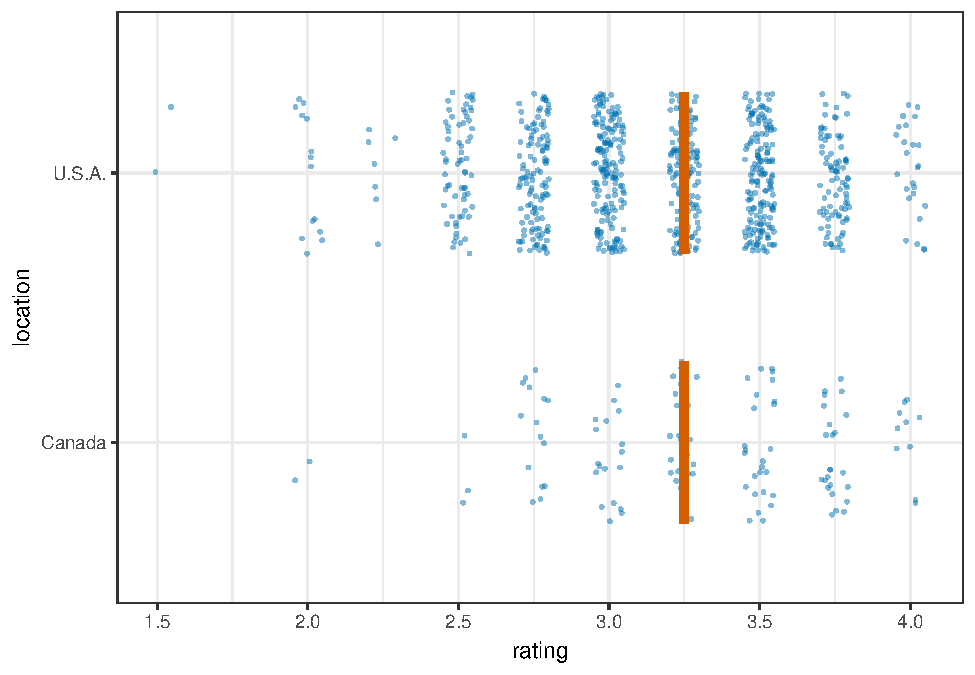
\includegraphics{Intro_Avensik_files/figure-latex/ungeviz-1.pdf} 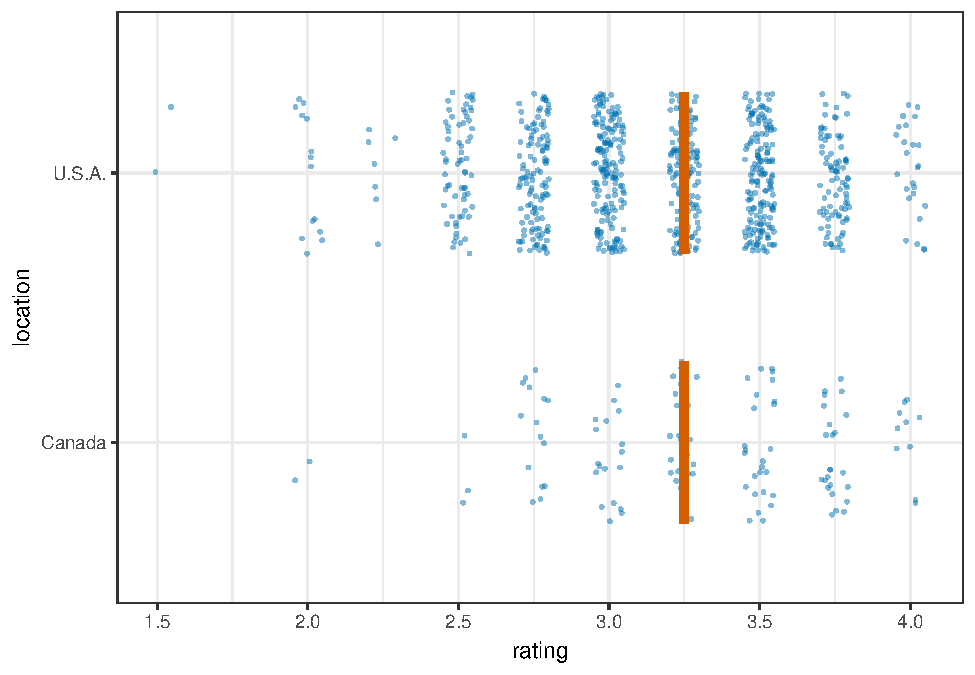
\includegraphics{Intro_Avensik_files/figure-latex/ungeviz-2.pdf} 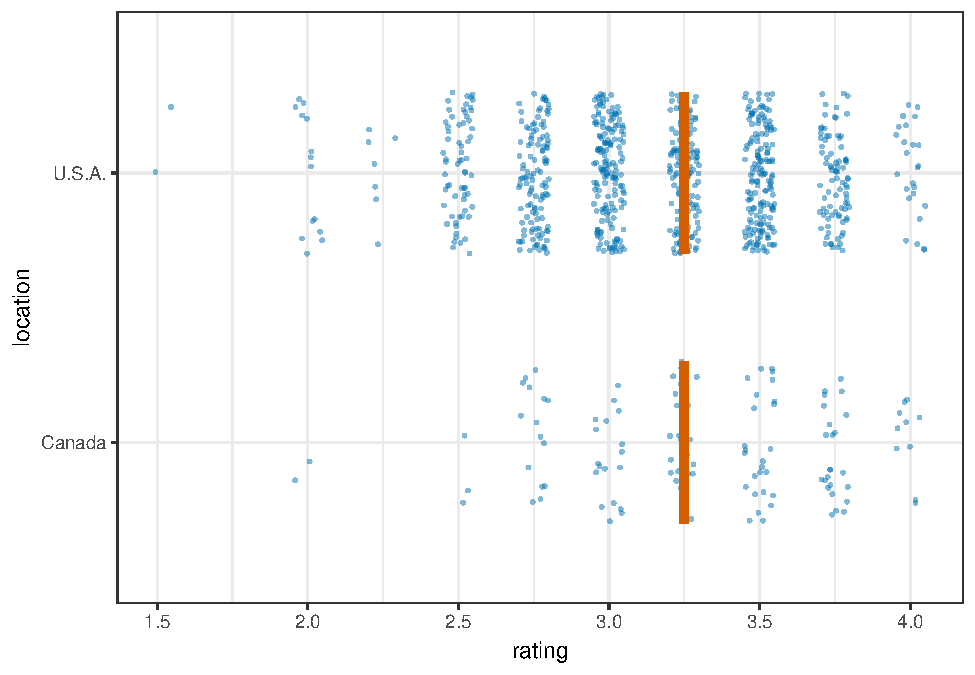
\includegraphics{Intro_Avensik_files/figure-latex/ungeviz-3.pdf} 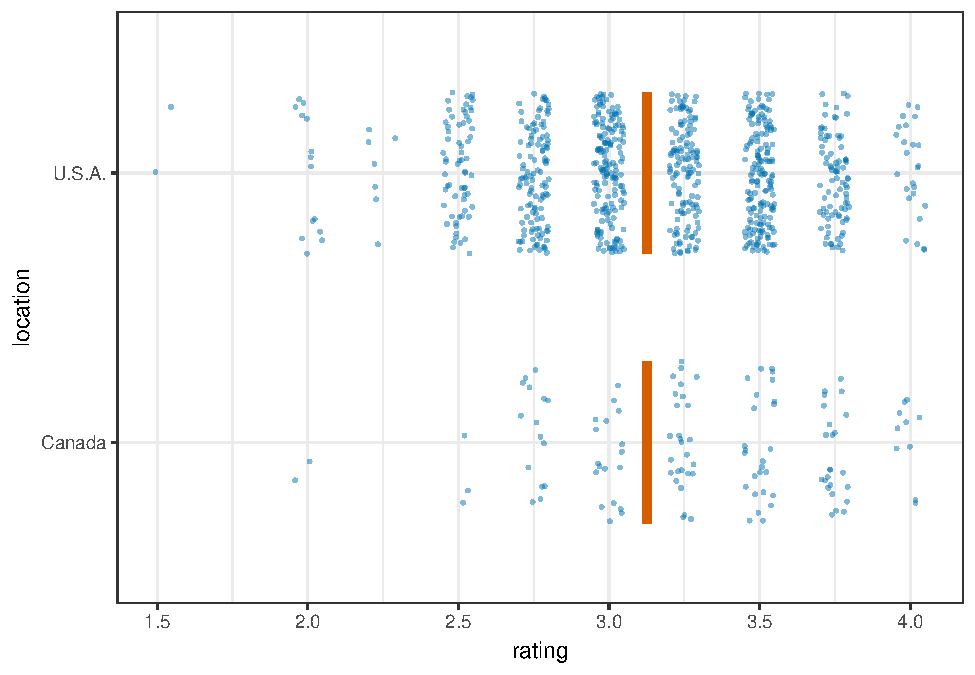
\includegraphics{Intro_Avensik_files/figure-latex/ungeviz-4.pdf} 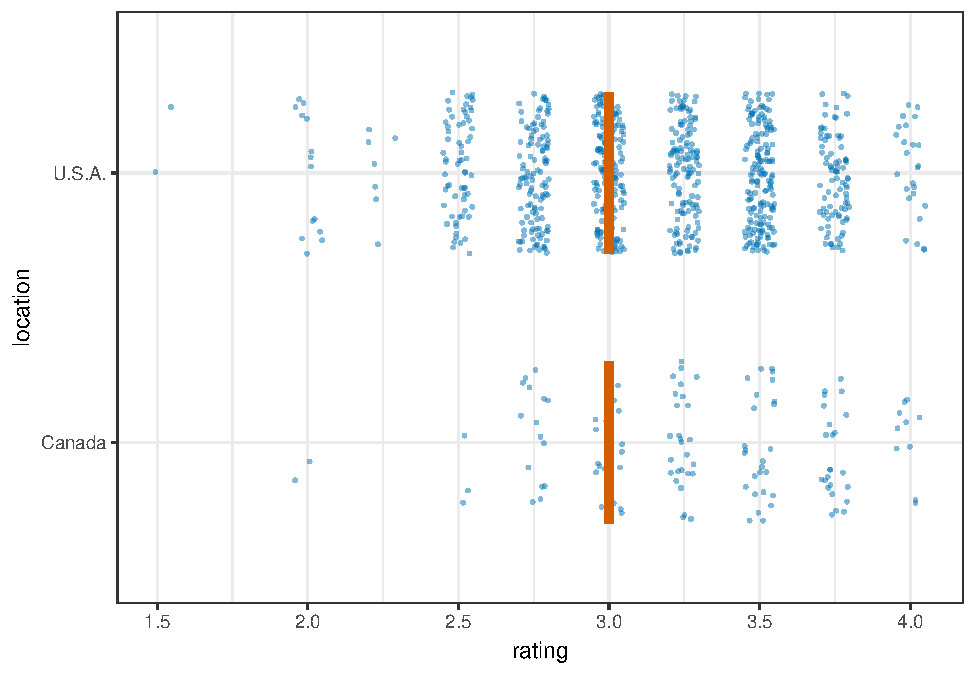
\includegraphics{Intro_Avensik_files/figure-latex/ungeviz-5.pdf} 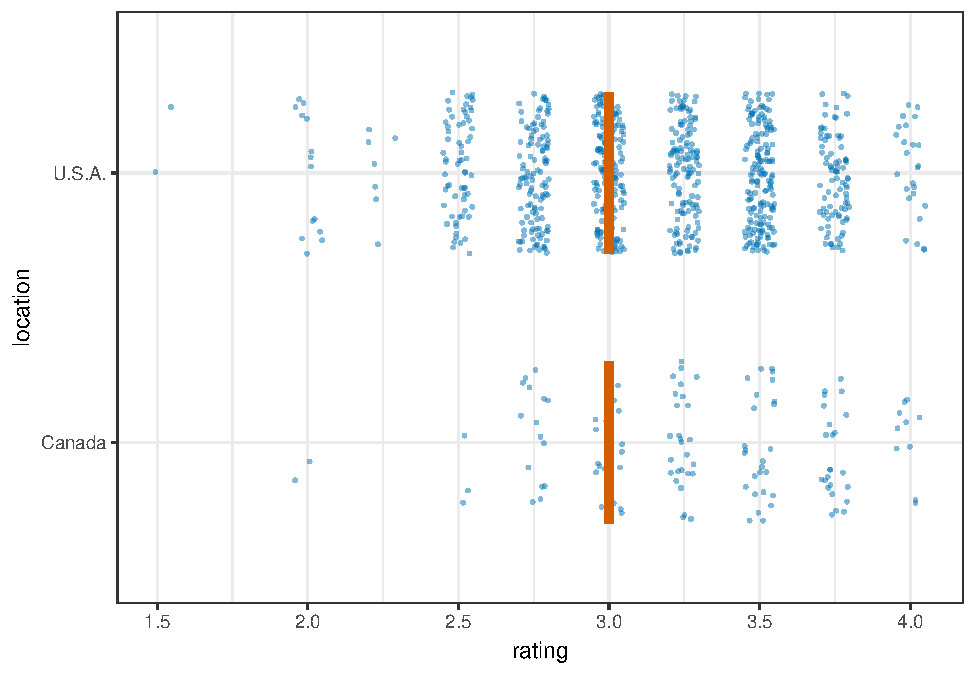
\includegraphics{Intro_Avensik_files/figure-latex/ungeviz-6.pdf} 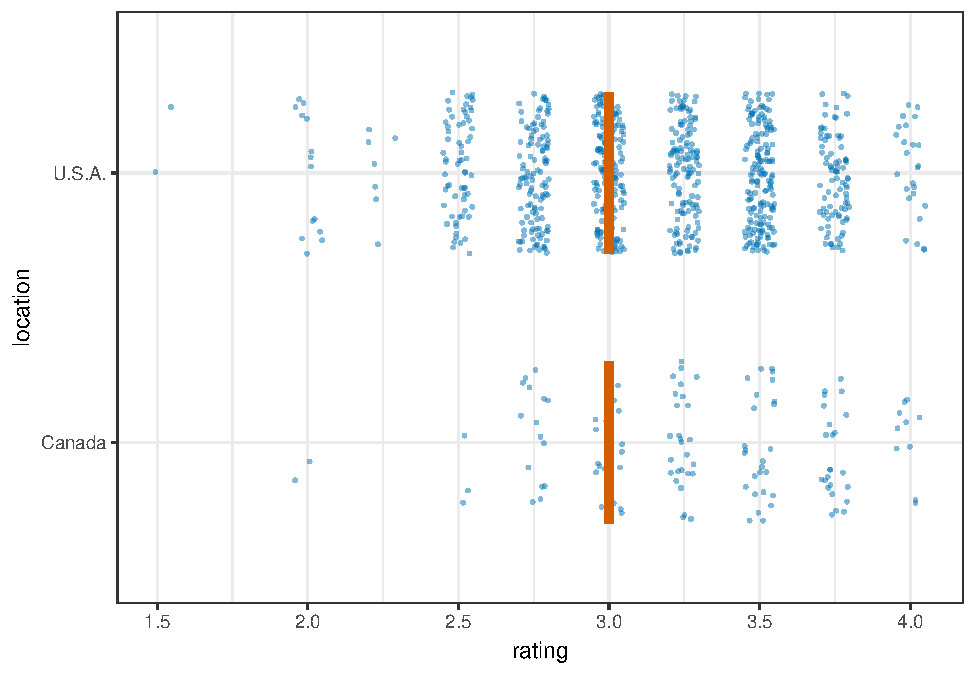
\includegraphics{Intro_Avensik_files/figure-latex/ungeviz-7.pdf} 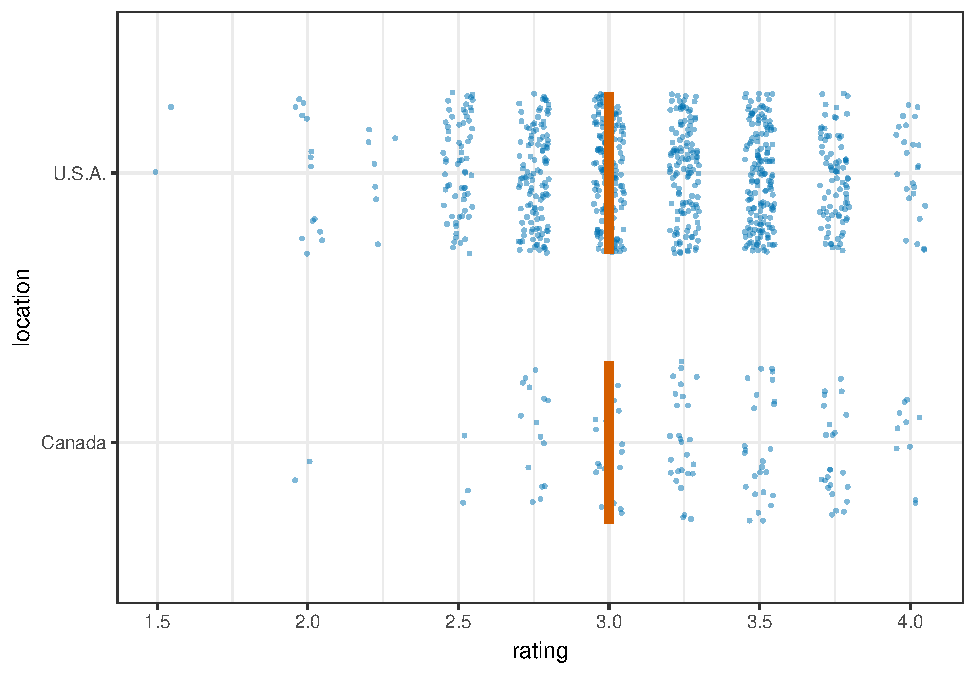
\includegraphics{Intro_Avensik_files/figure-latex/ungeviz-8.pdf} 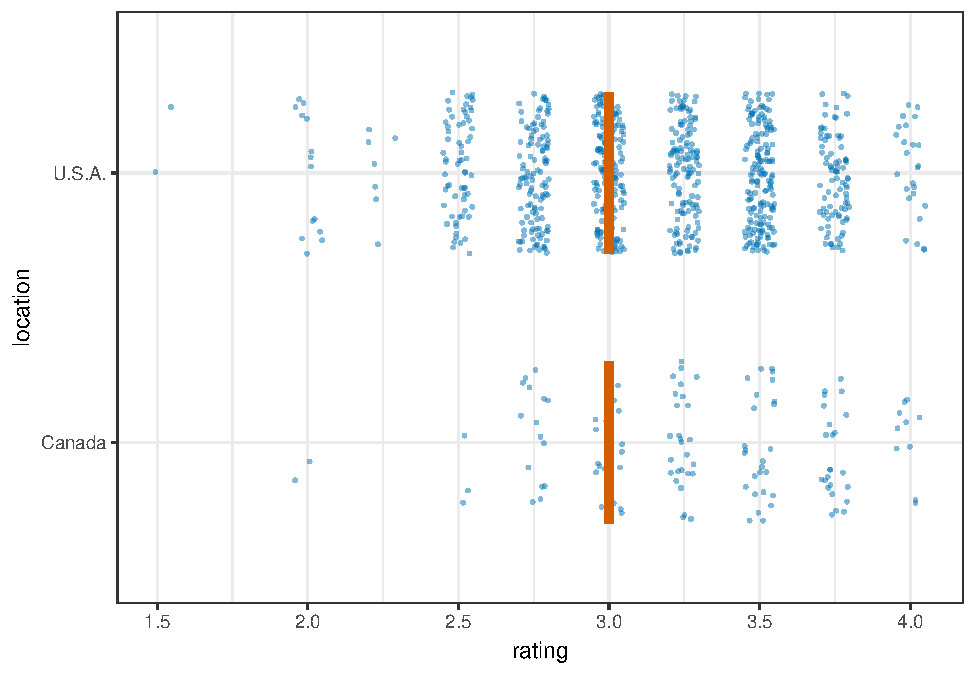
\includegraphics{Intro_Avensik_files/figure-latex/ungeviz-9.pdf} 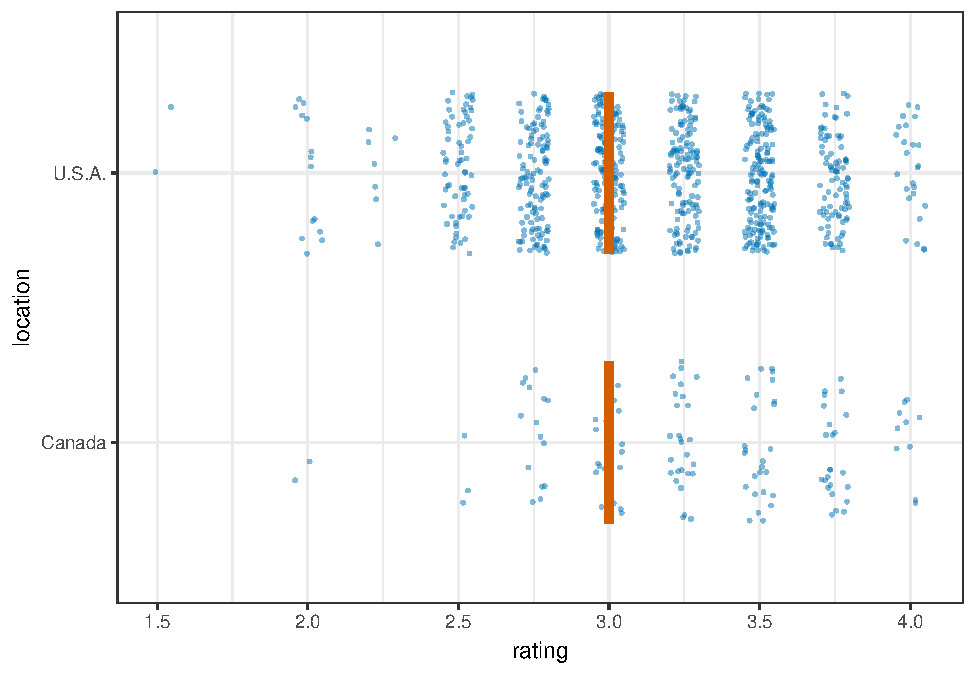
\includegraphics{Intro_Avensik_files/figure-latex/ungeviz-10.pdf} 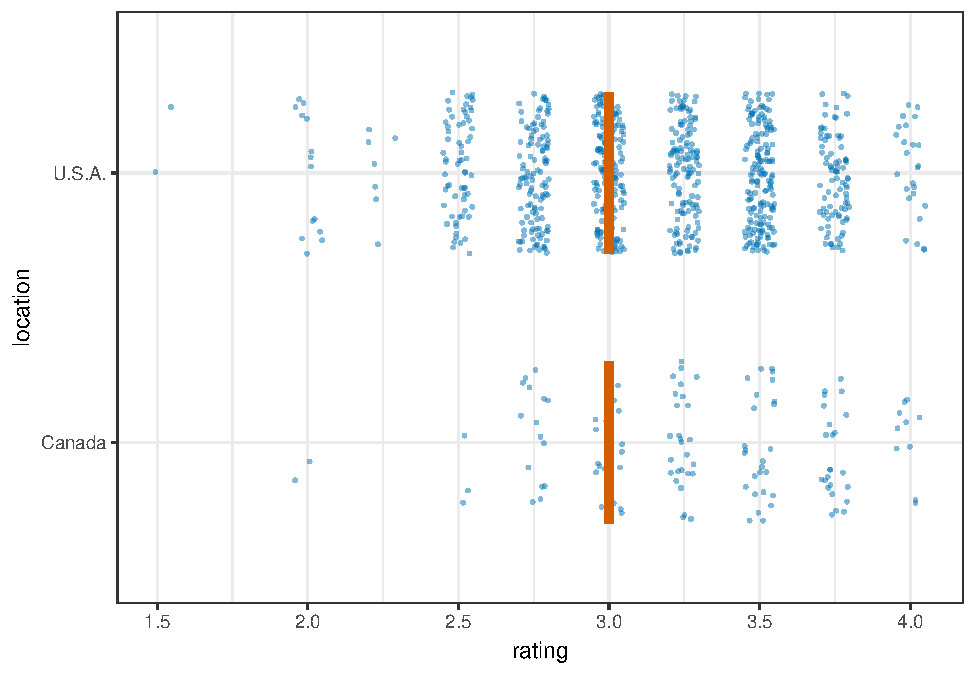
\includegraphics{Intro_Avensik_files/figure-latex/ungeviz-11.pdf} 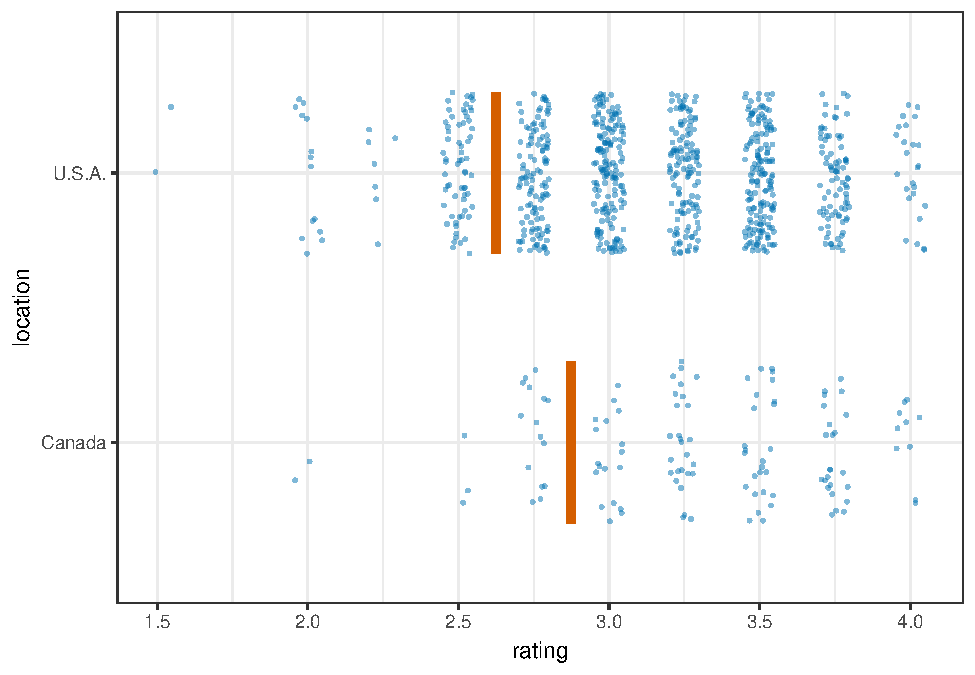
\includegraphics{Intro_Avensik_files/figure-latex/ungeviz-12.pdf} 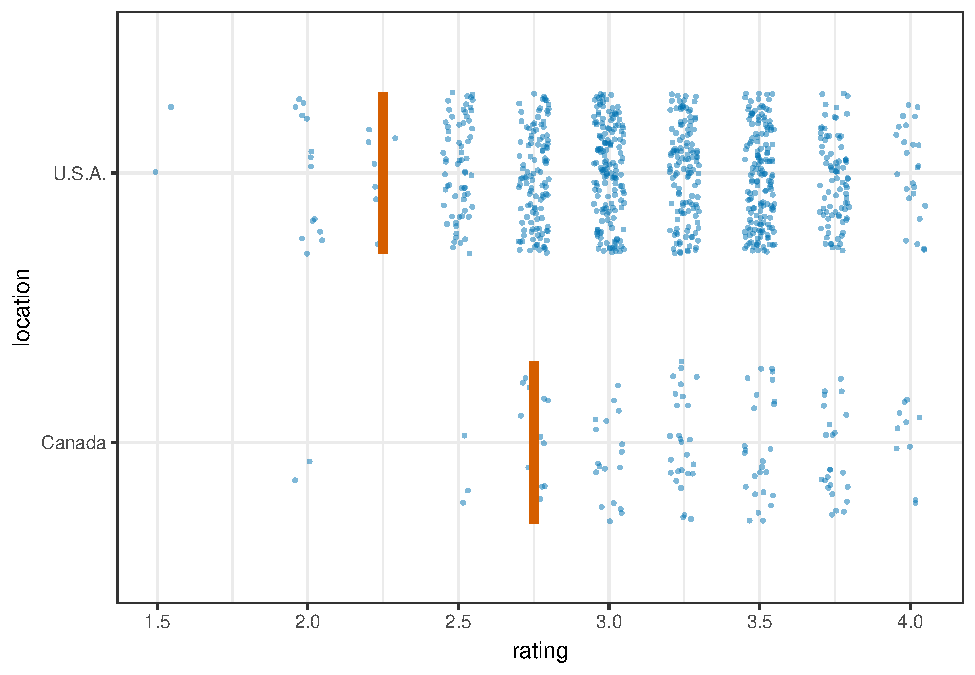
\includegraphics{Intro_Avensik_files/figure-latex/ungeviz-13.pdf} 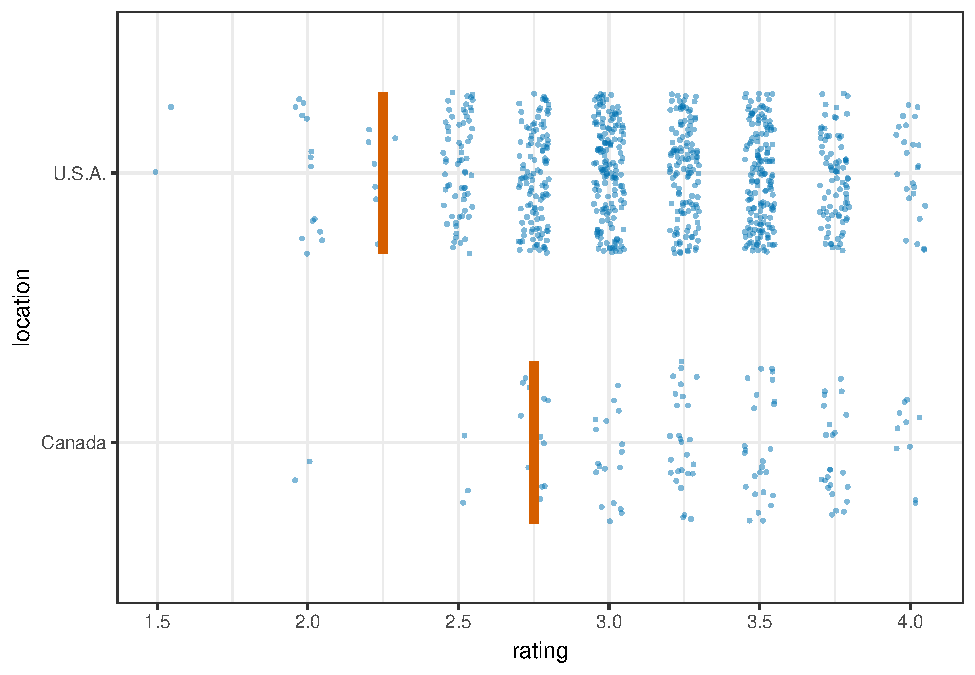
\includegraphics{Intro_Avensik_files/figure-latex/ungeviz-14.pdf} 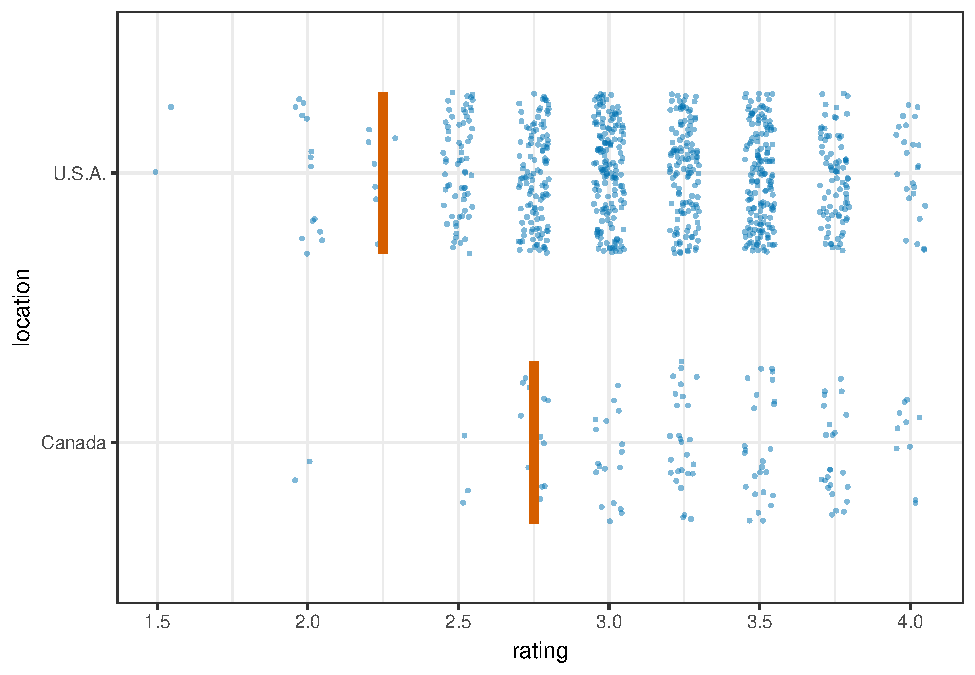
\includegraphics{Intro_Avensik_files/figure-latex/ungeviz-15.pdf} 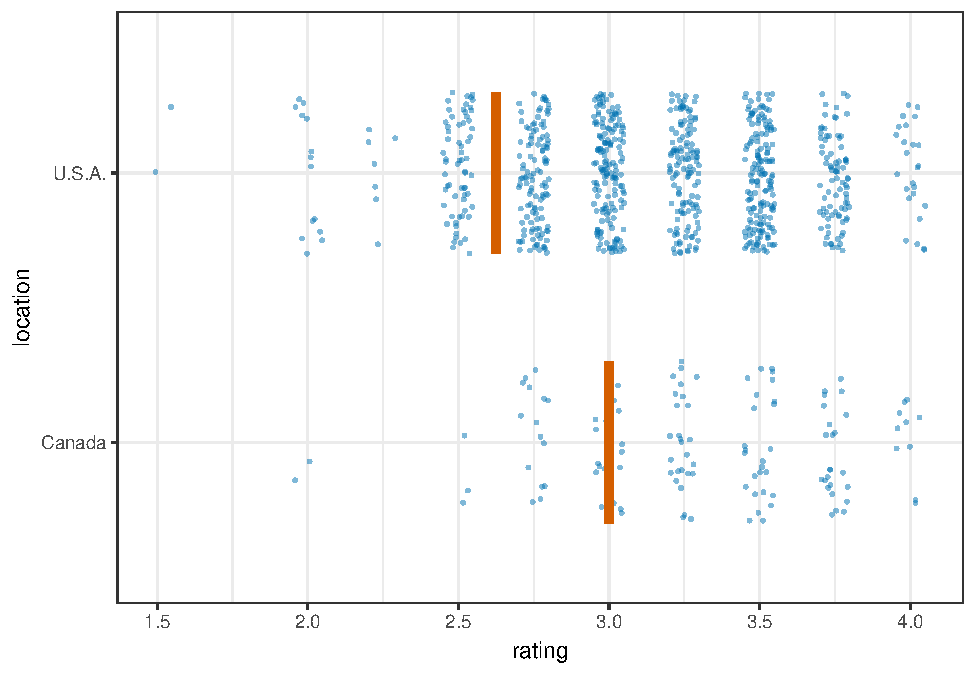
\includegraphics{Intro_Avensik_files/figure-latex/ungeviz-16.pdf} 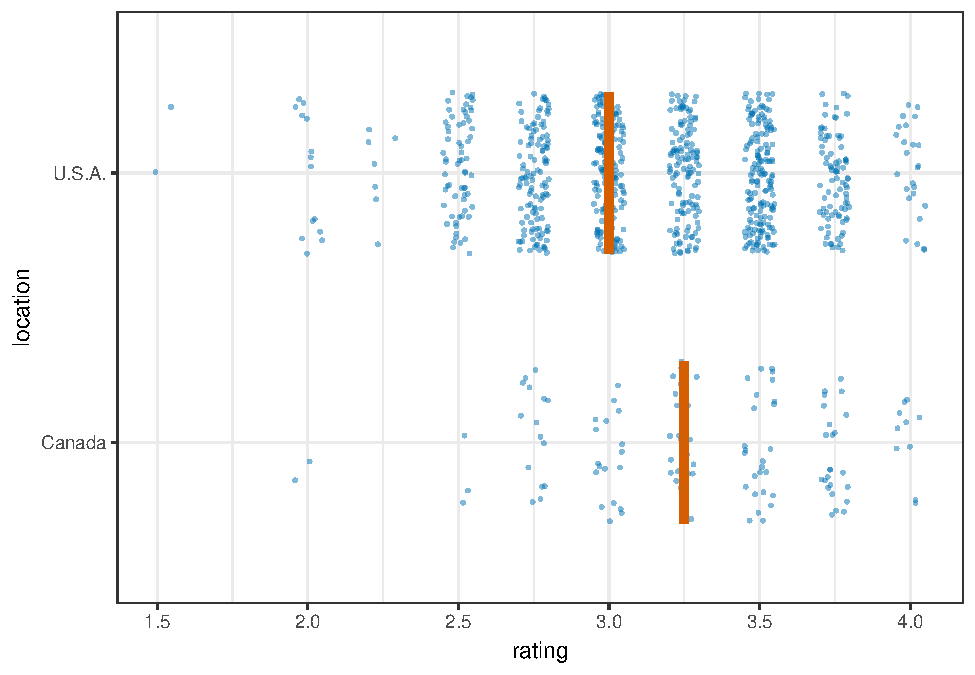
\includegraphics{Intro_Avensik_files/figure-latex/ungeviz-17.pdf} 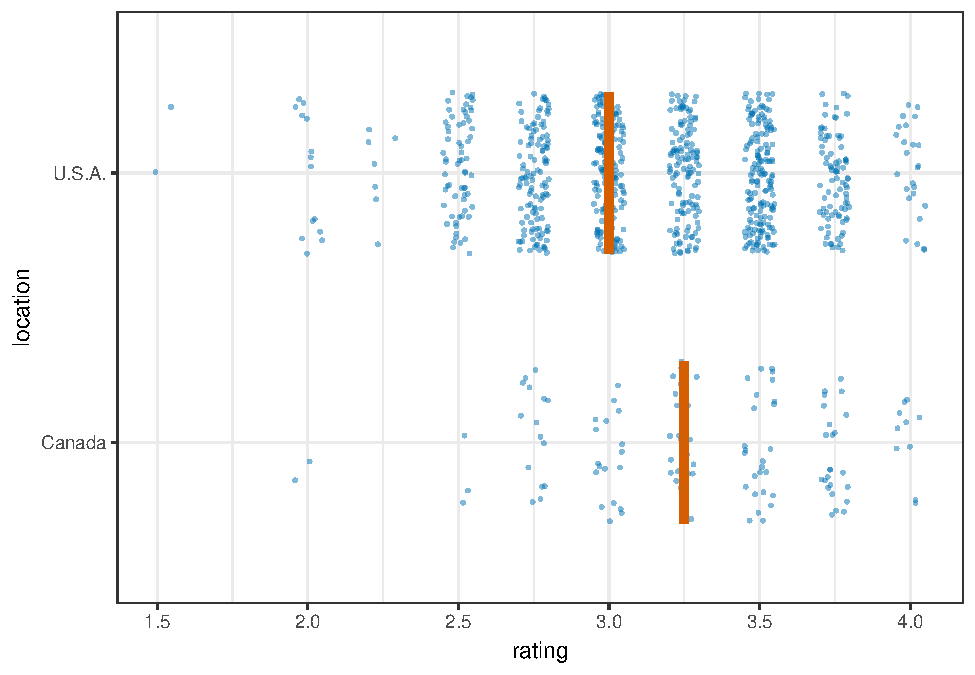
\includegraphics{Intro_Avensik_files/figure-latex/ungeviz-18.pdf} 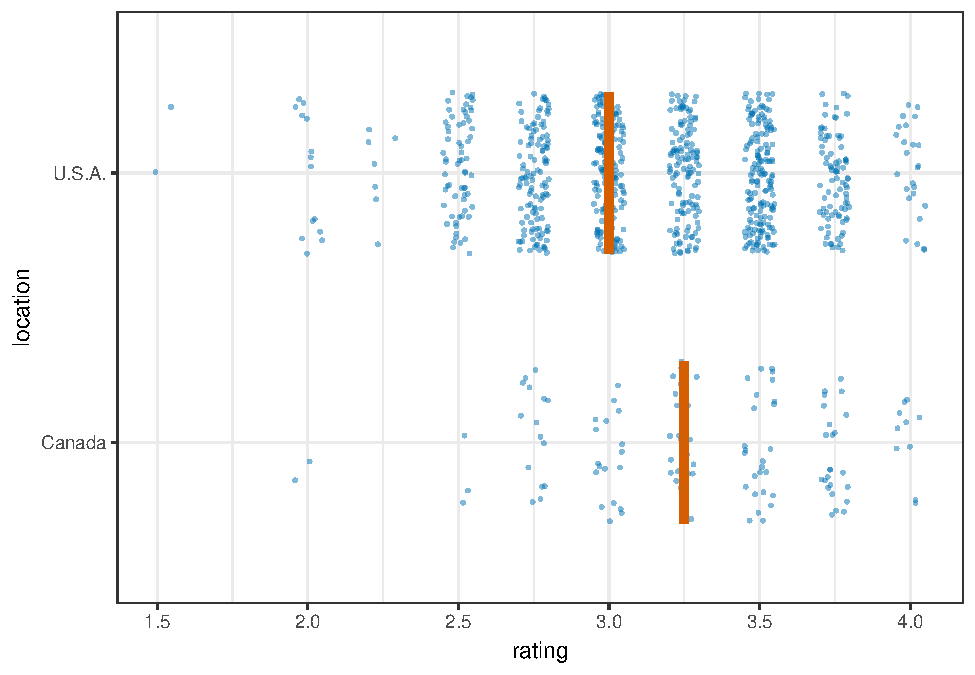
\includegraphics{Intro_Avensik_files/figure-latex/ungeviz-19.pdf} 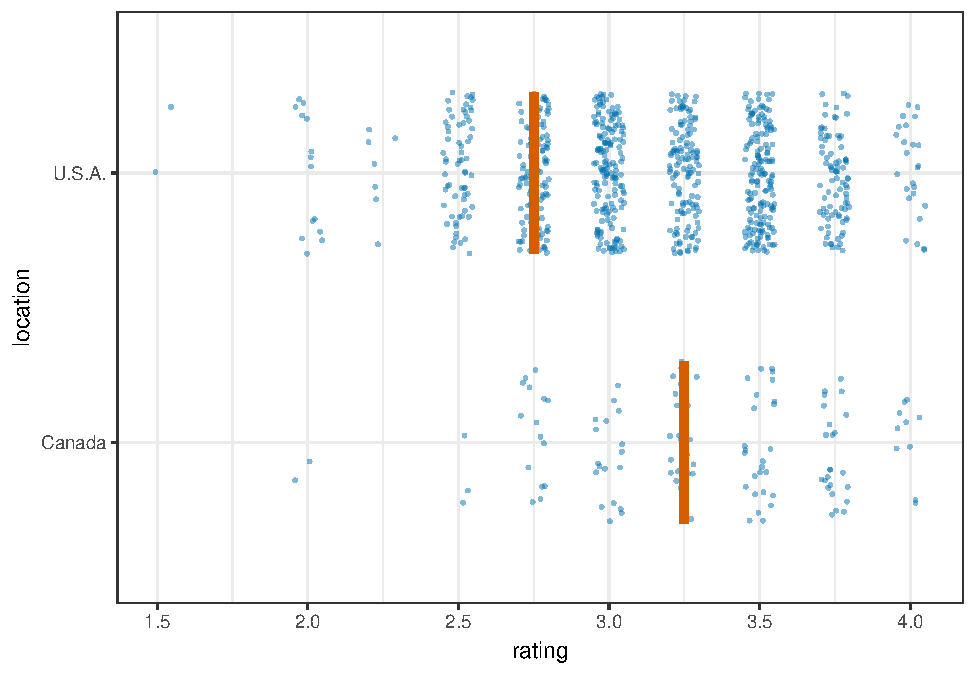
\includegraphics{Intro_Avensik_files/figure-latex/ungeviz-20.pdf} 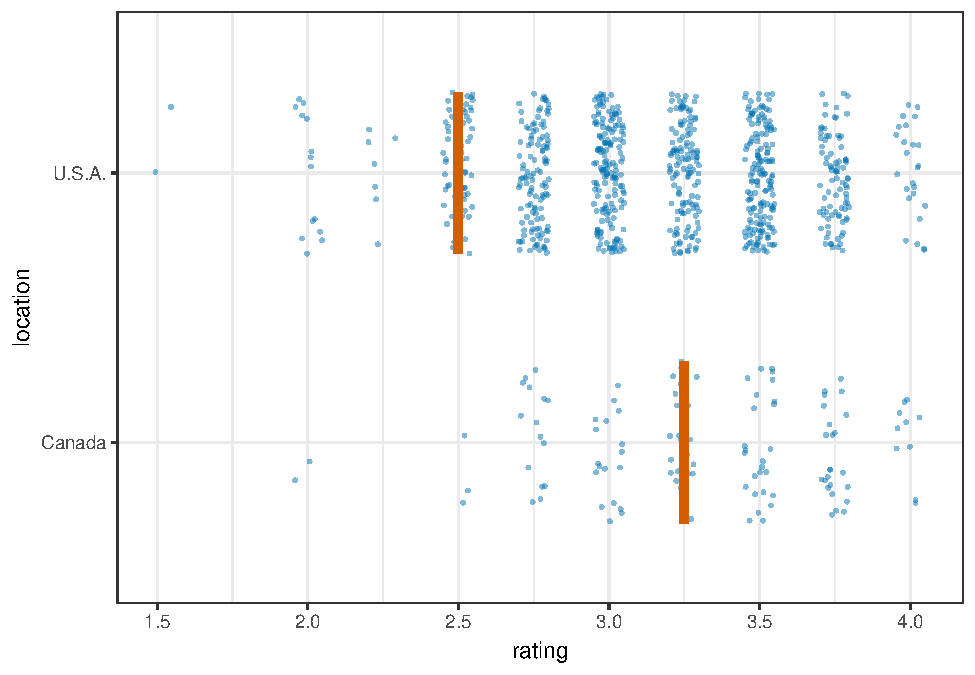
\includegraphics{Intro_Avensik_files/figure-latex/ungeviz-21.pdf} 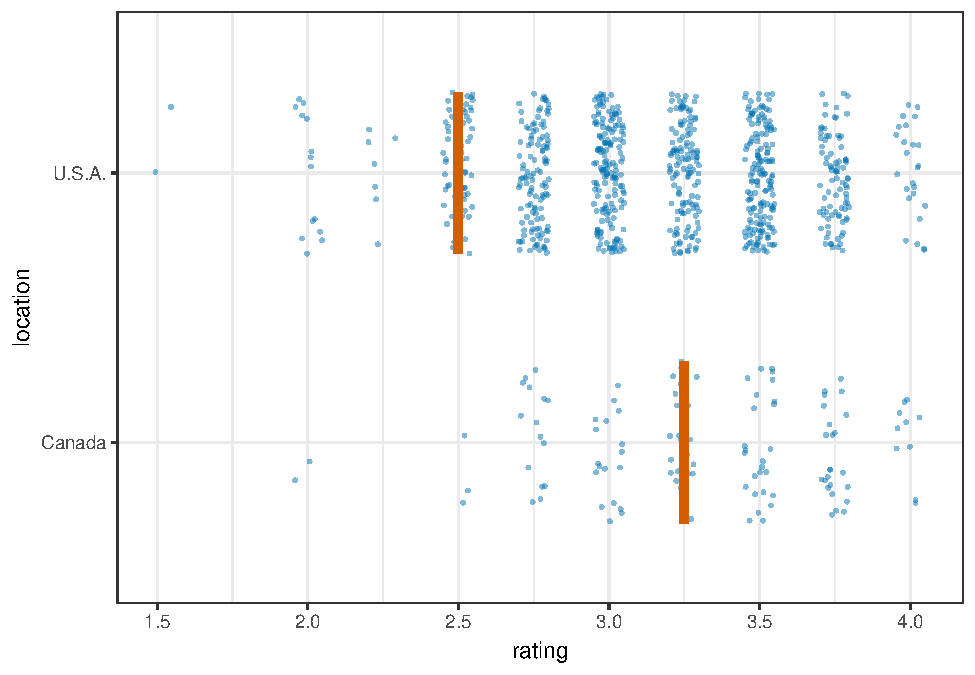
\includegraphics{Intro_Avensik_files/figure-latex/ungeviz-22.pdf} 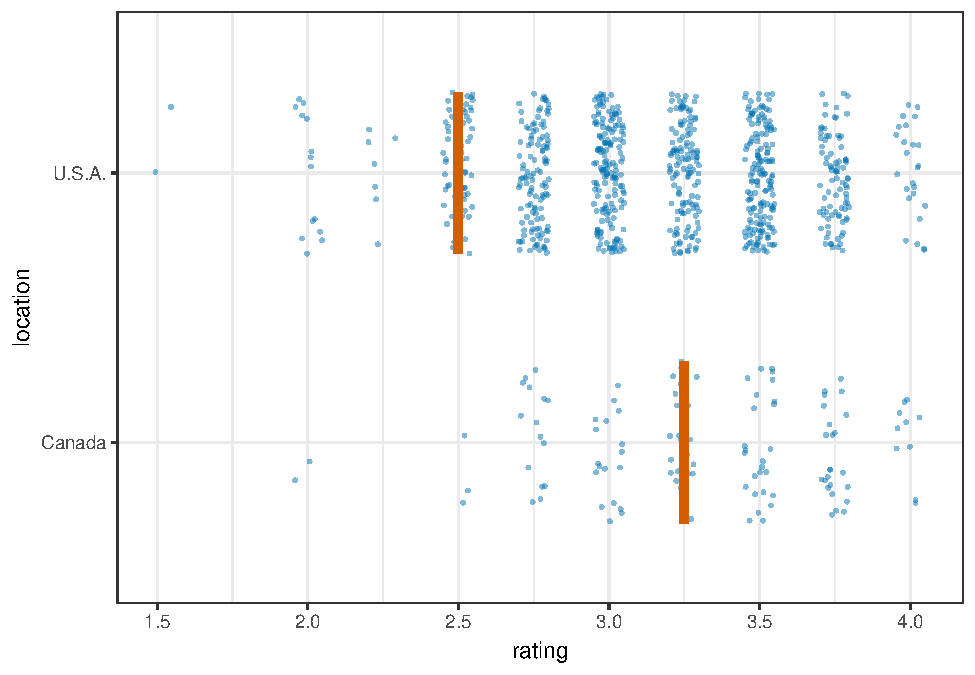
\includegraphics{Intro_Avensik_files/figure-latex/ungeviz-23.pdf} 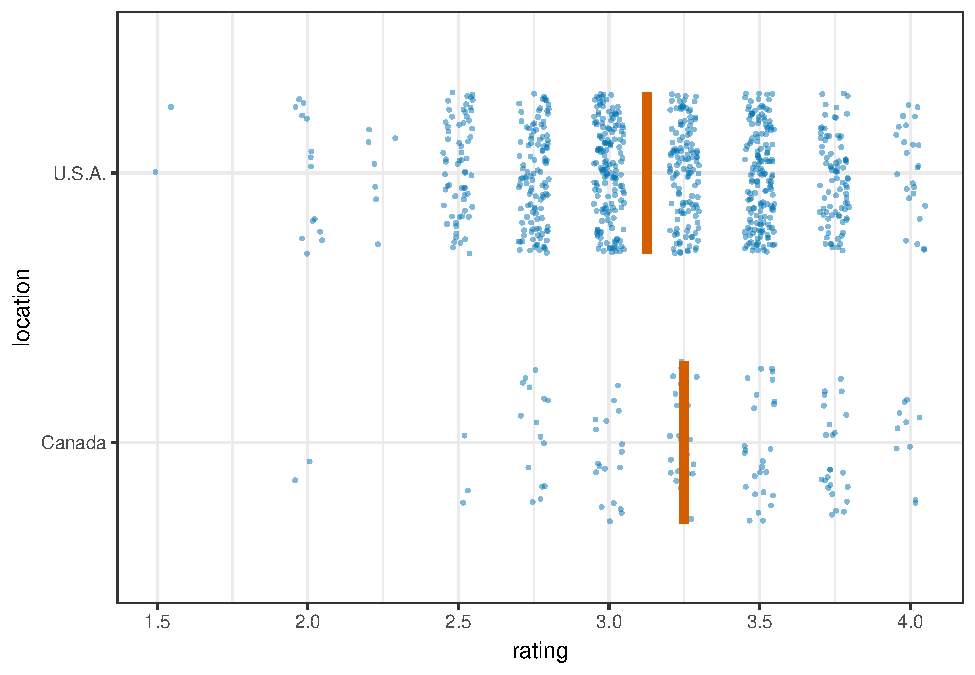
\includegraphics{Intro_Avensik_files/figure-latex/ungeviz-24.pdf} 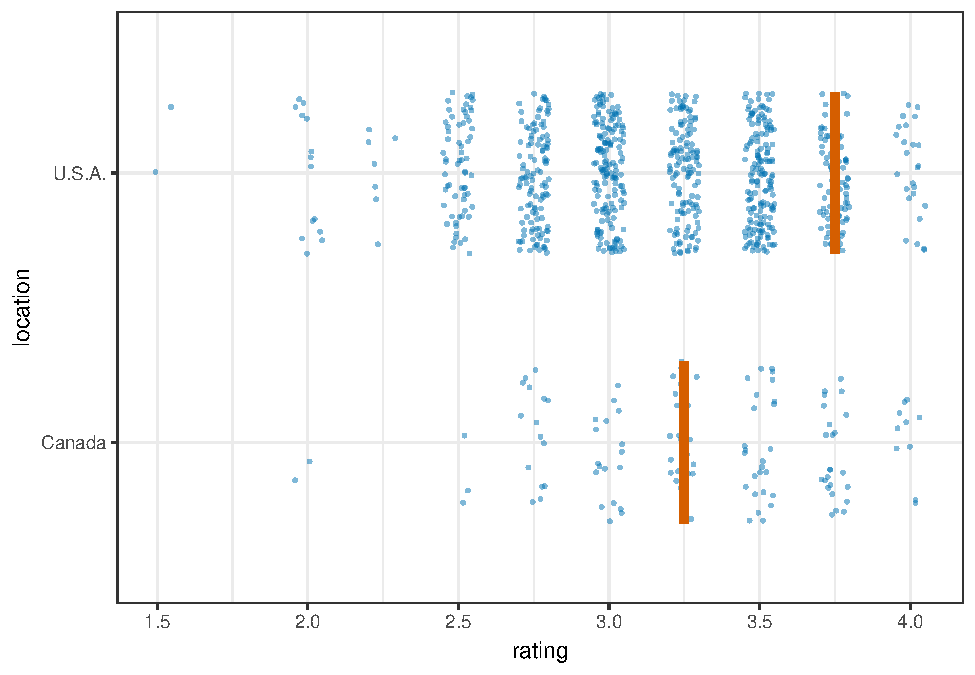
\includegraphics{Intro_Avensik_files/figure-latex/ungeviz-25.pdf} 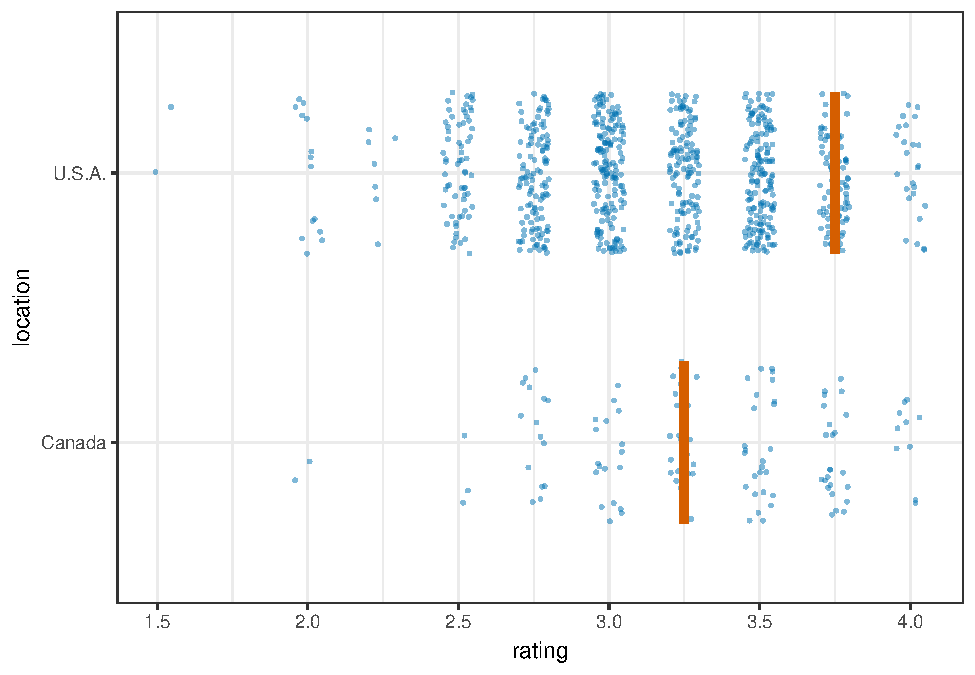
\includegraphics{Intro_Avensik_files/figure-latex/ungeviz-26.pdf} 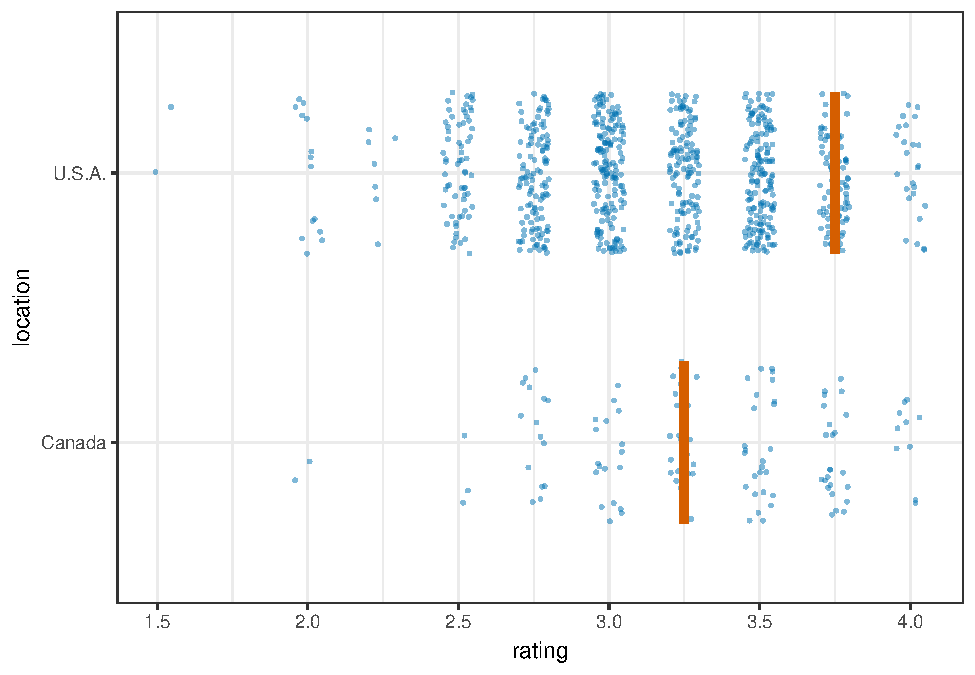
\includegraphics{Intro_Avensik_files/figure-latex/ungeviz-27.pdf} 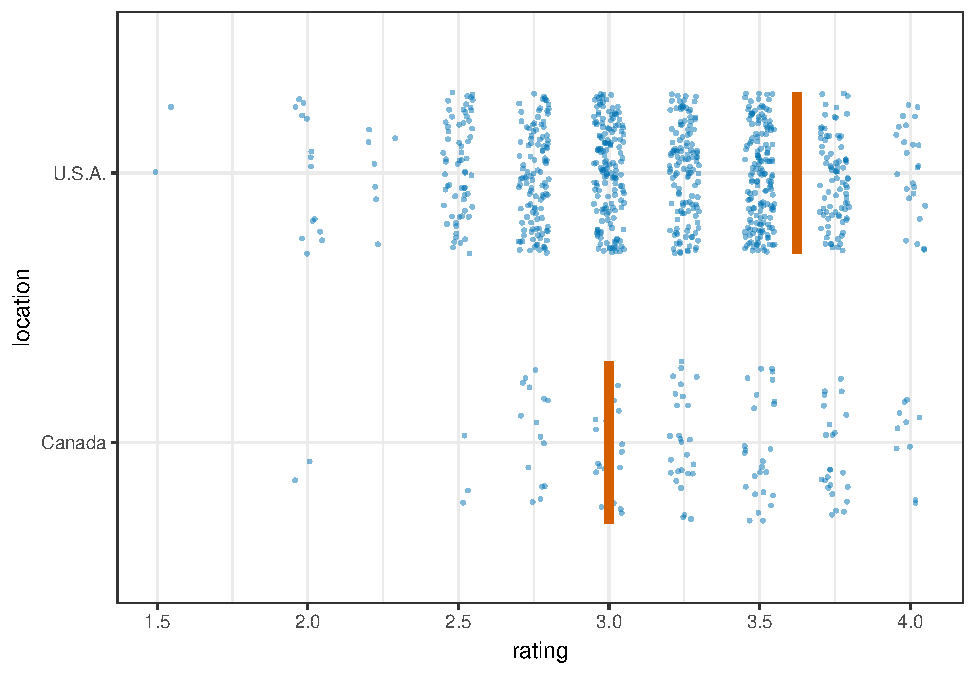
\includegraphics{Intro_Avensik_files/figure-latex/ungeviz-28.pdf} 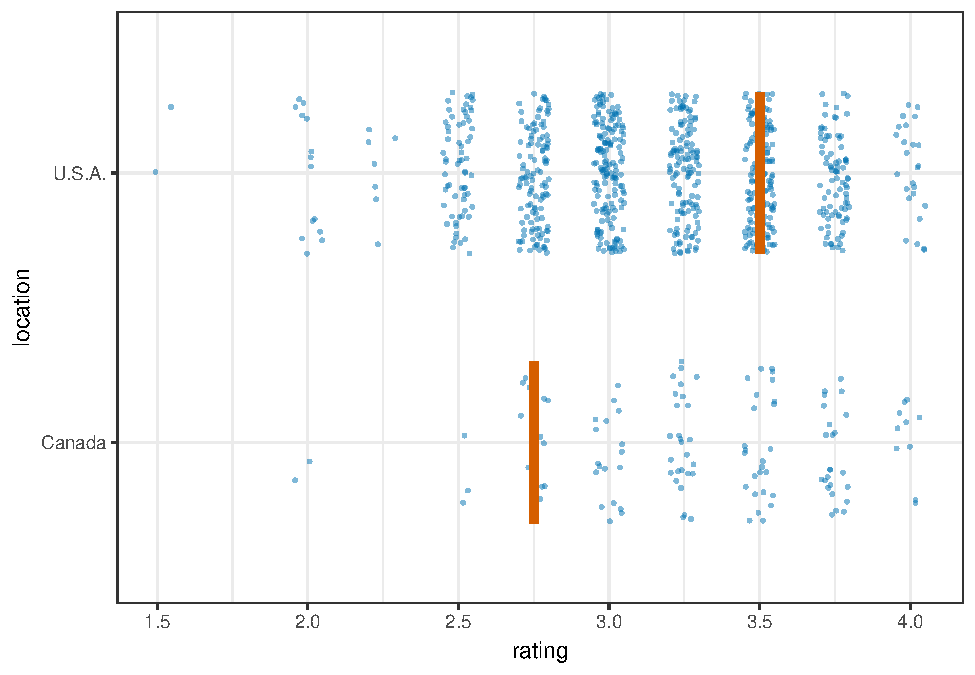
\includegraphics{Intro_Avensik_files/figure-latex/ungeviz-29.pdf} 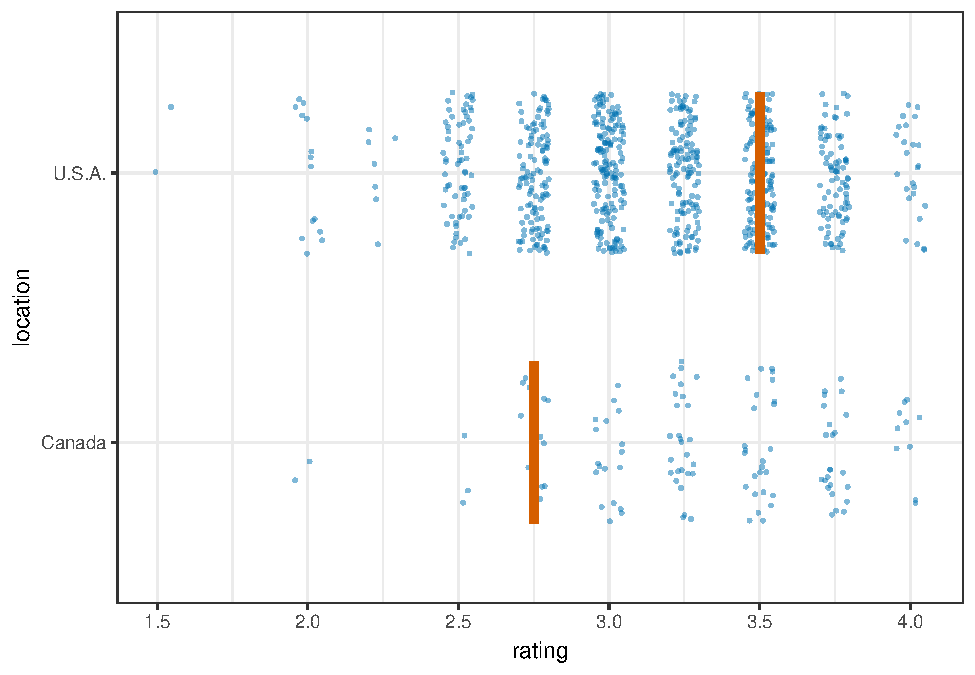
\includegraphics{Intro_Avensik_files/figure-latex/ungeviz-30.pdf} 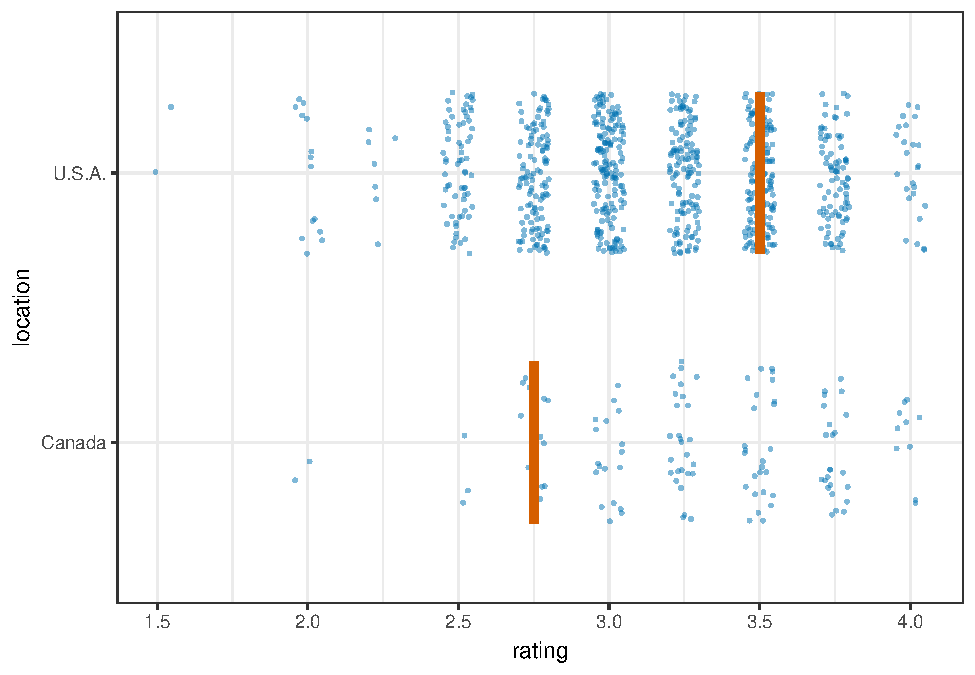
\includegraphics{Intro_Avensik_files/figure-latex/ungeviz-31.pdf} 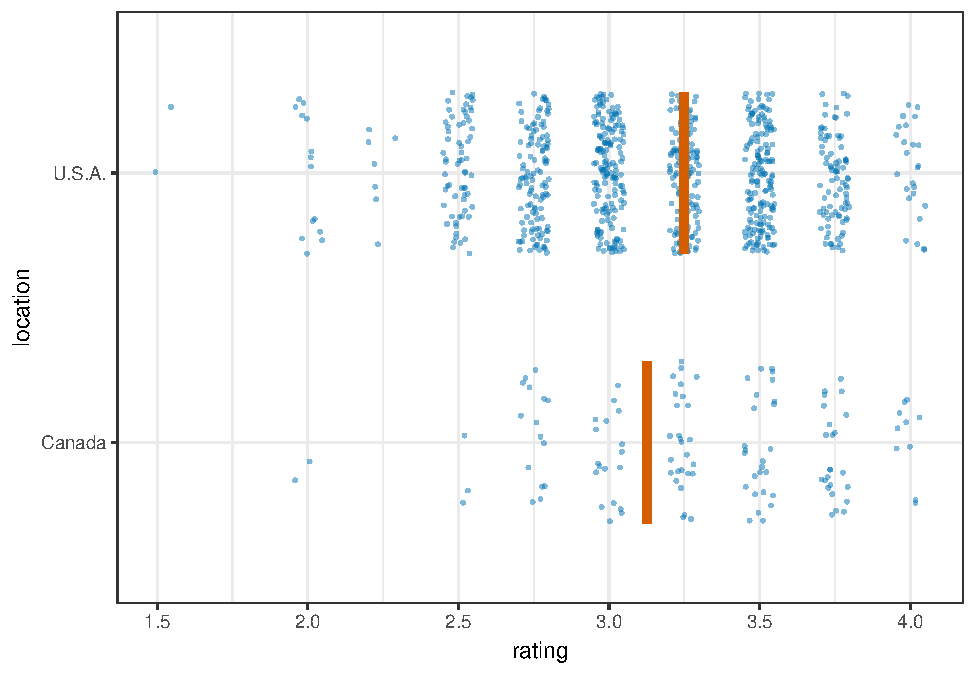
\includegraphics{Intro_Avensik_files/figure-latex/ungeviz-32.pdf} 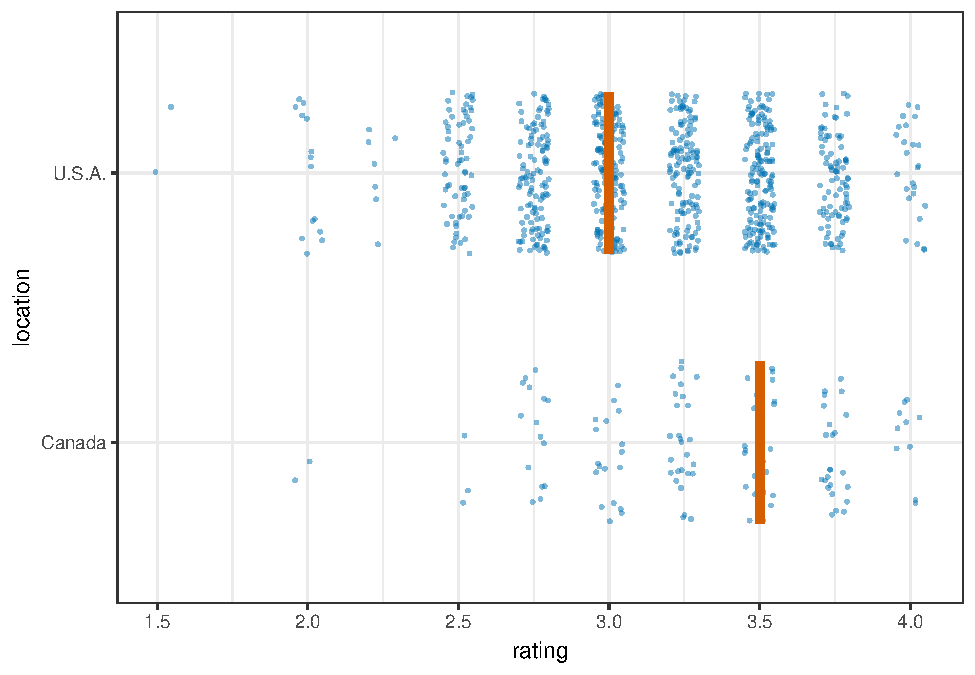
\includegraphics{Intro_Avensik_files/figure-latex/ungeviz-33.pdf} 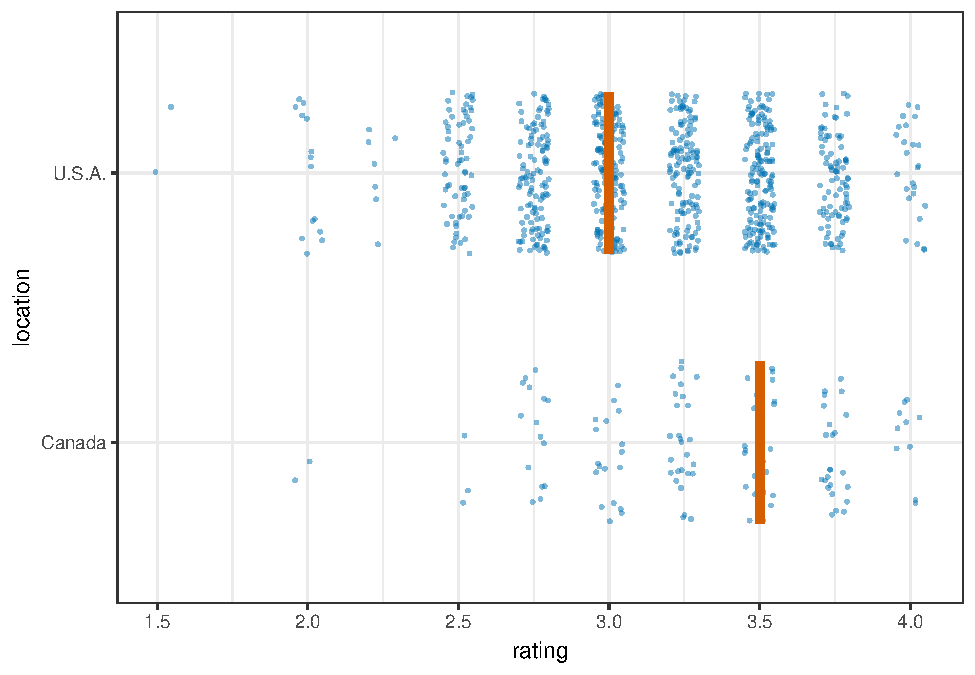
\includegraphics{Intro_Avensik_files/figure-latex/ungeviz-34.pdf} 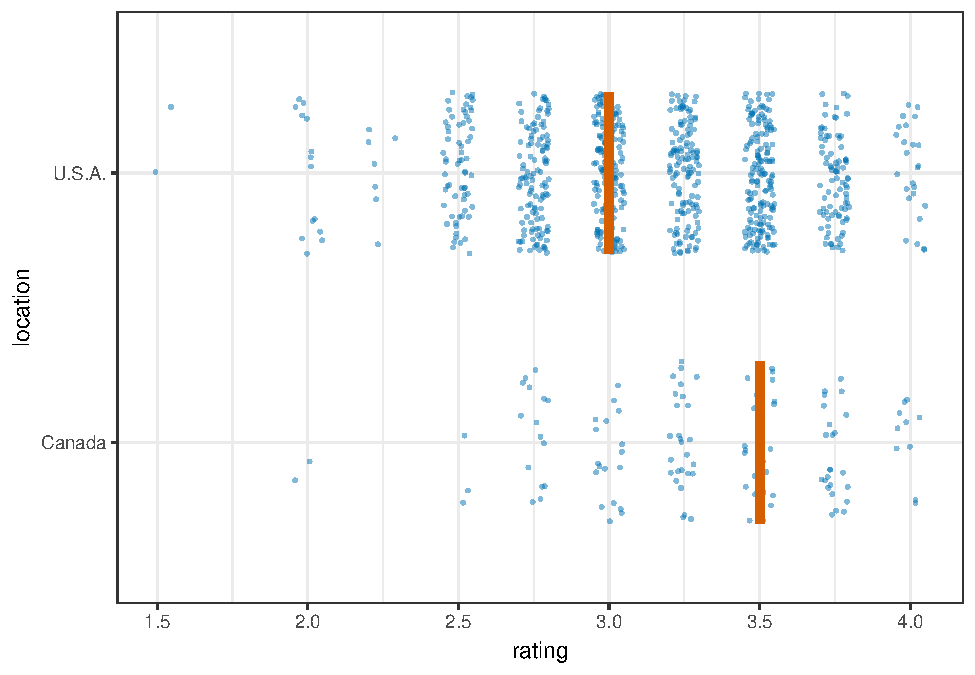
\includegraphics{Intro_Avensik_files/figure-latex/ungeviz-35.pdf} 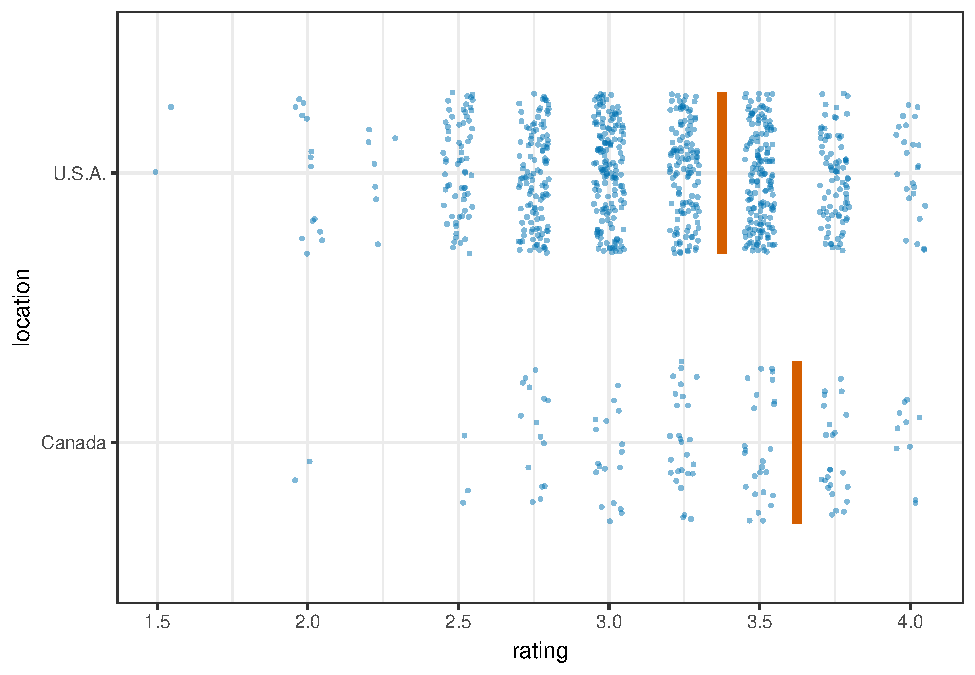
\includegraphics{Intro_Avensik_files/figure-latex/ungeviz-36.pdf} 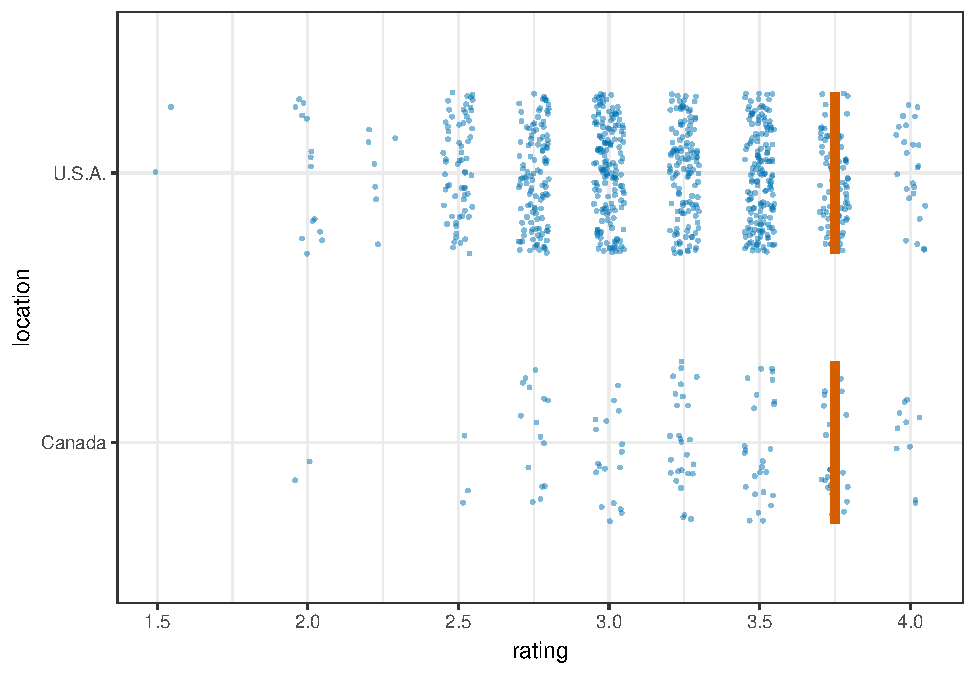
\includegraphics{Intro_Avensik_files/figure-latex/ungeviz-37.pdf} 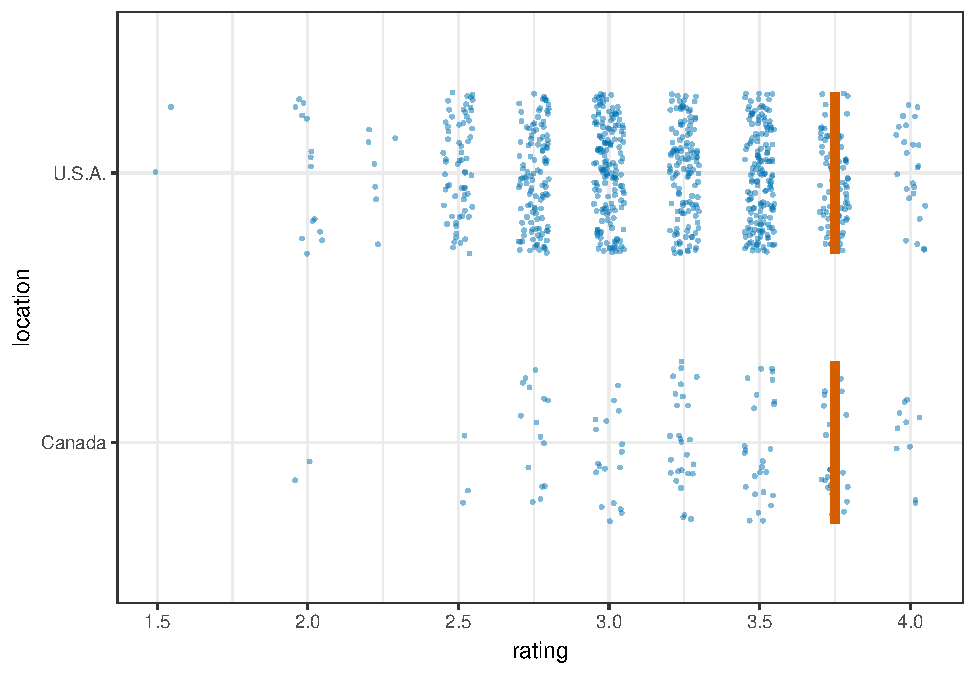
\includegraphics{Intro_Avensik_files/figure-latex/ungeviz-38.pdf} 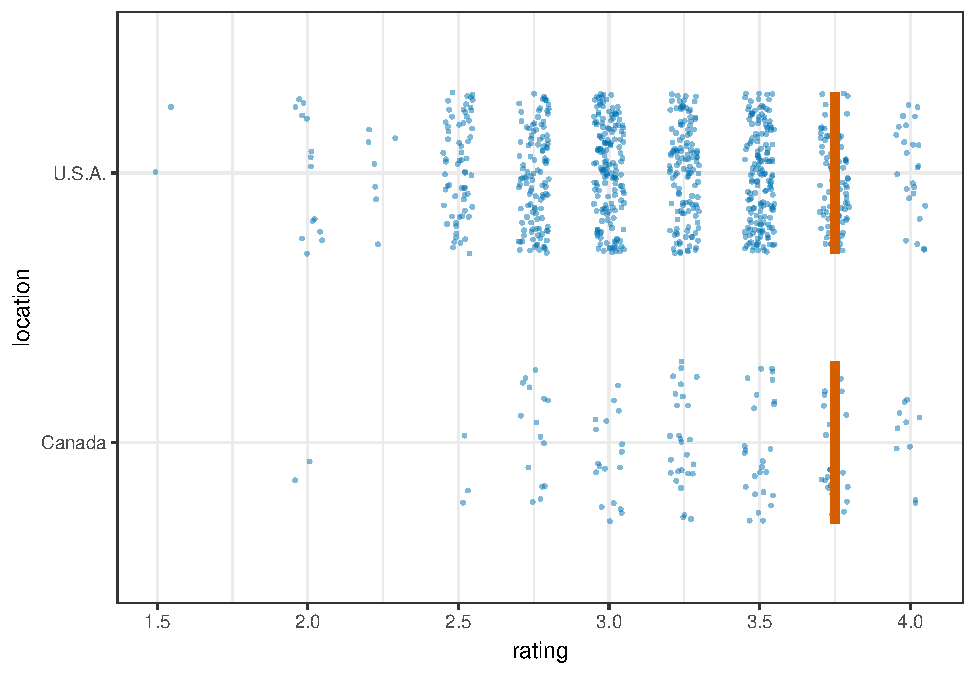
\includegraphics{Intro_Avensik_files/figure-latex/ungeviz-39.pdf} 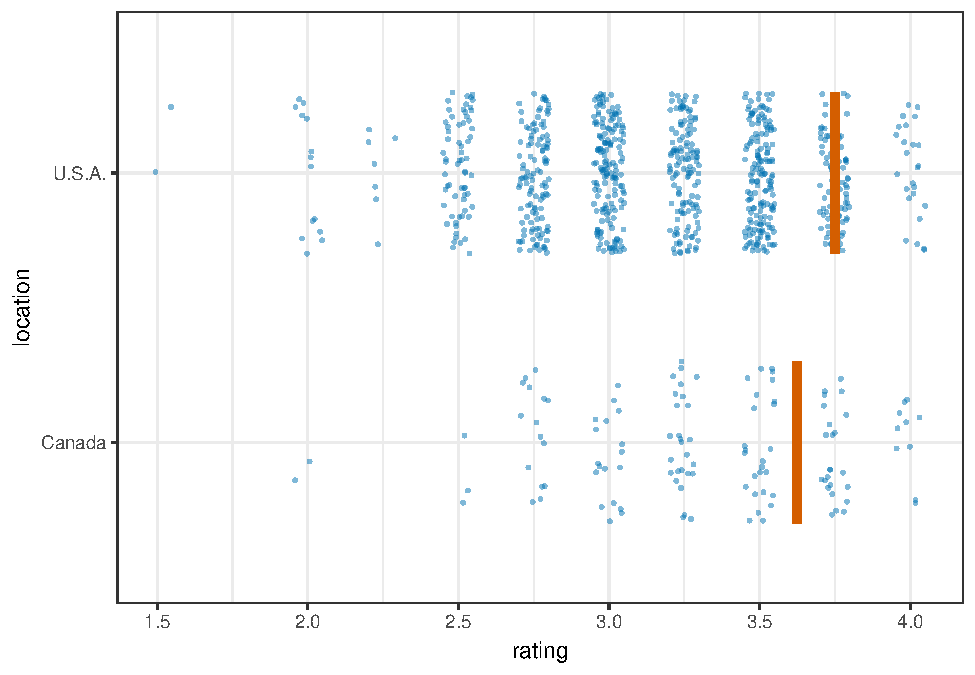
\includegraphics{Intro_Avensik_files/figure-latex/ungeviz-40.pdf} 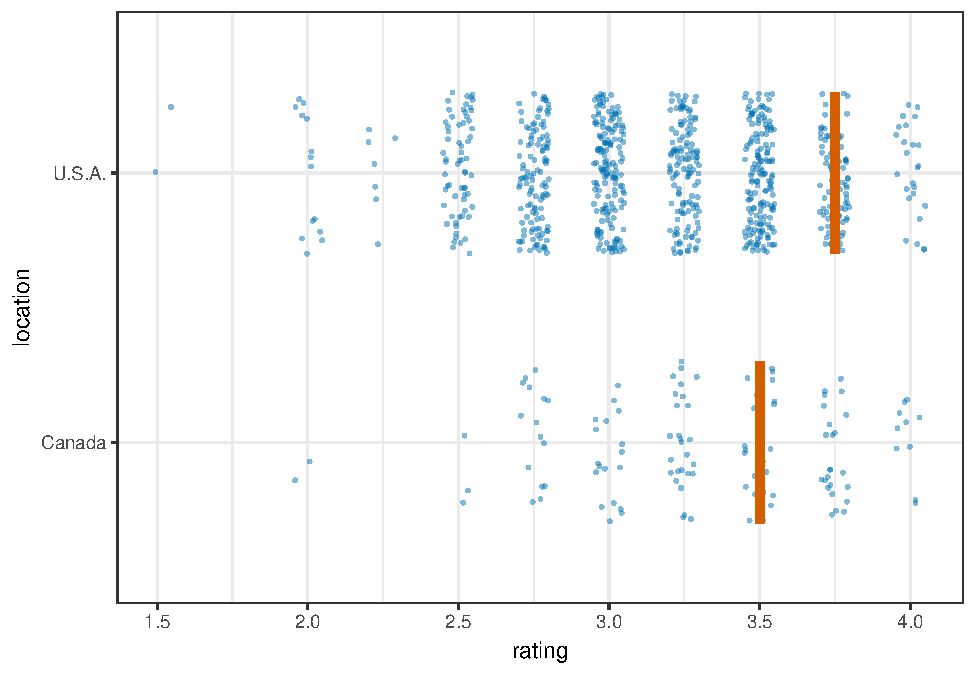
\includegraphics{Intro_Avensik_files/figure-latex/ungeviz-41.pdf} 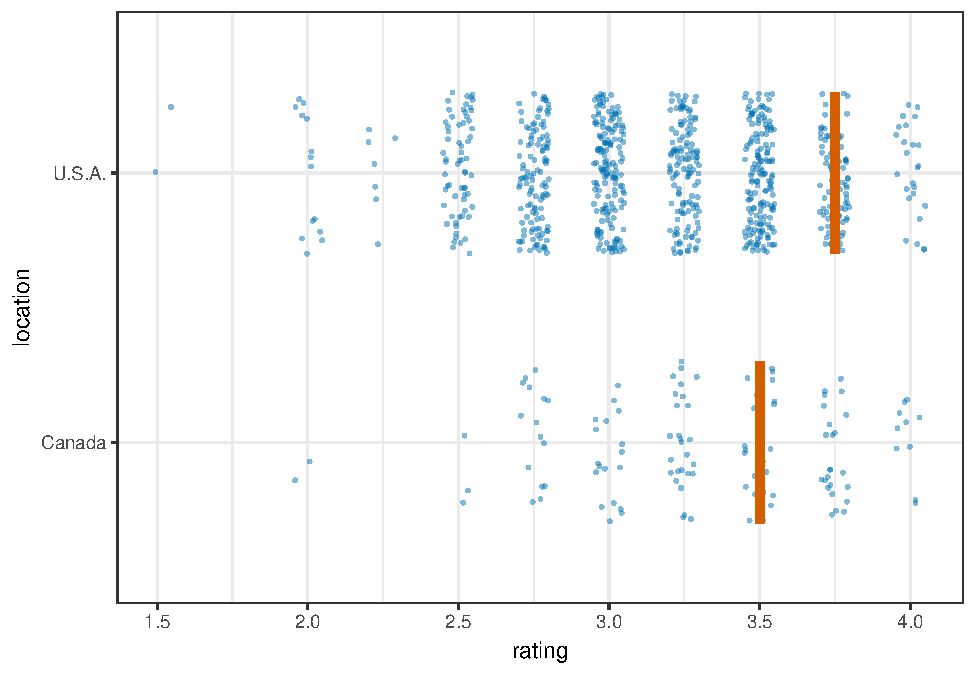
\includegraphics{Intro_Avensik_files/figure-latex/ungeviz-42.pdf} 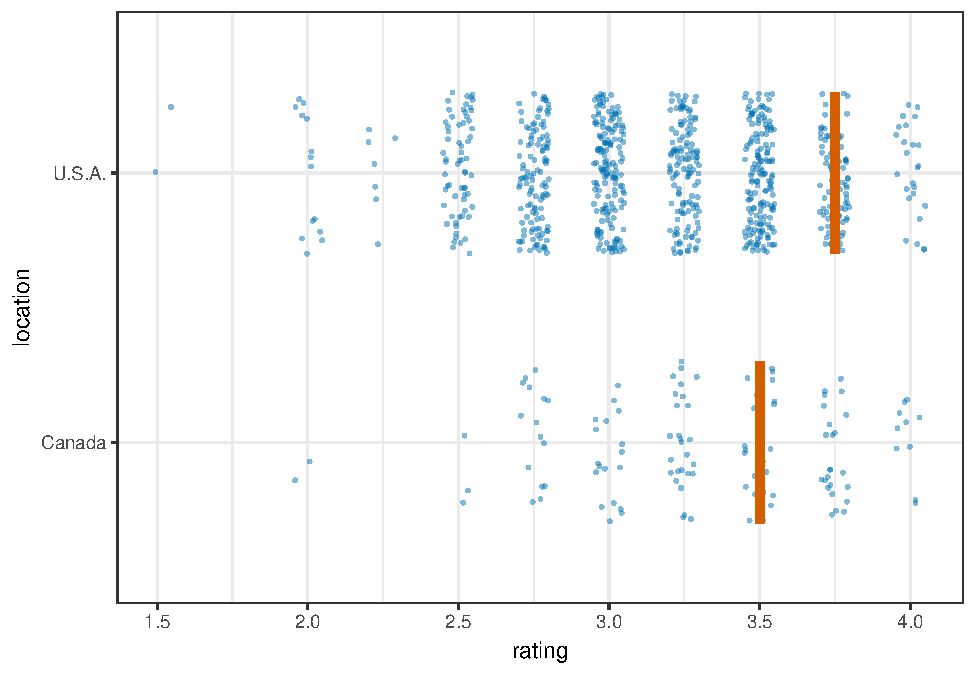
\includegraphics{Intro_Avensik_files/figure-latex/ungeviz-43.pdf} 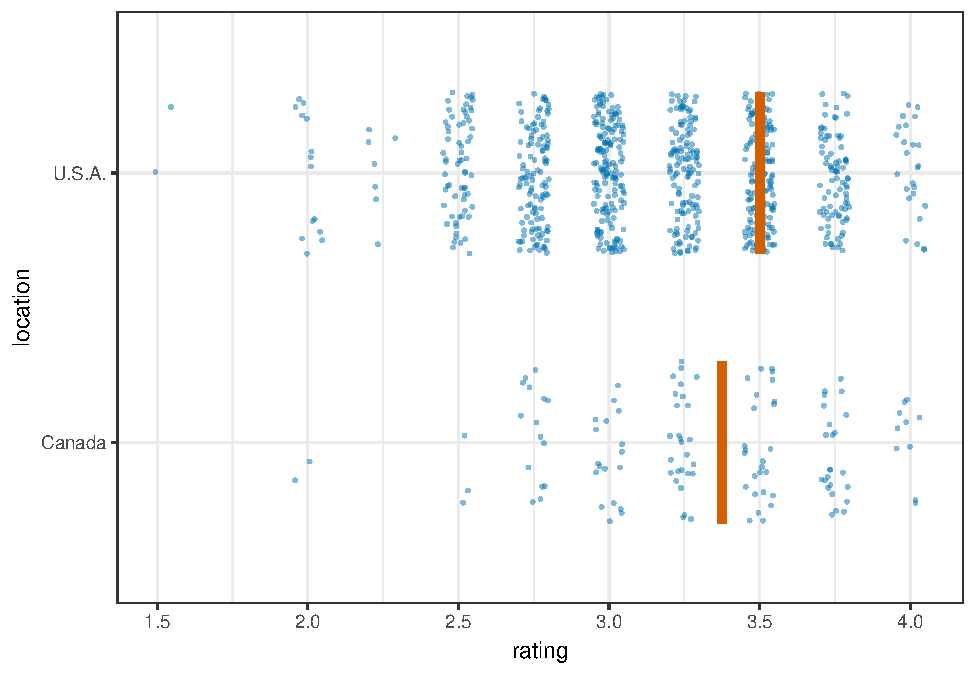
\includegraphics{Intro_Avensik_files/figure-latex/ungeviz-44.pdf} 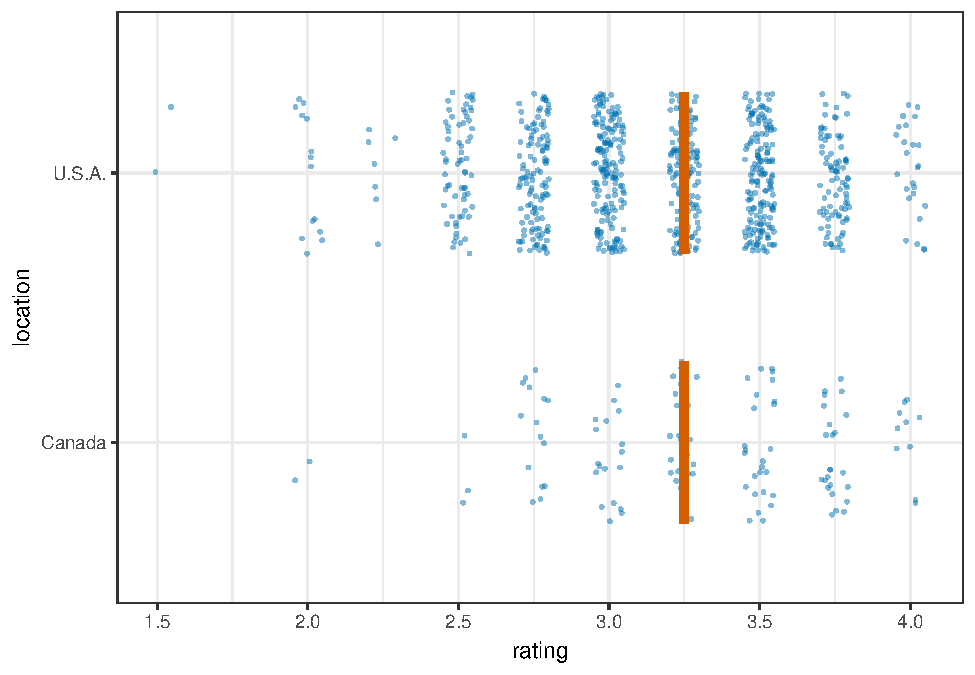
\includegraphics{Intro_Avensik_files/figure-latex/ungeviz-45.pdf} 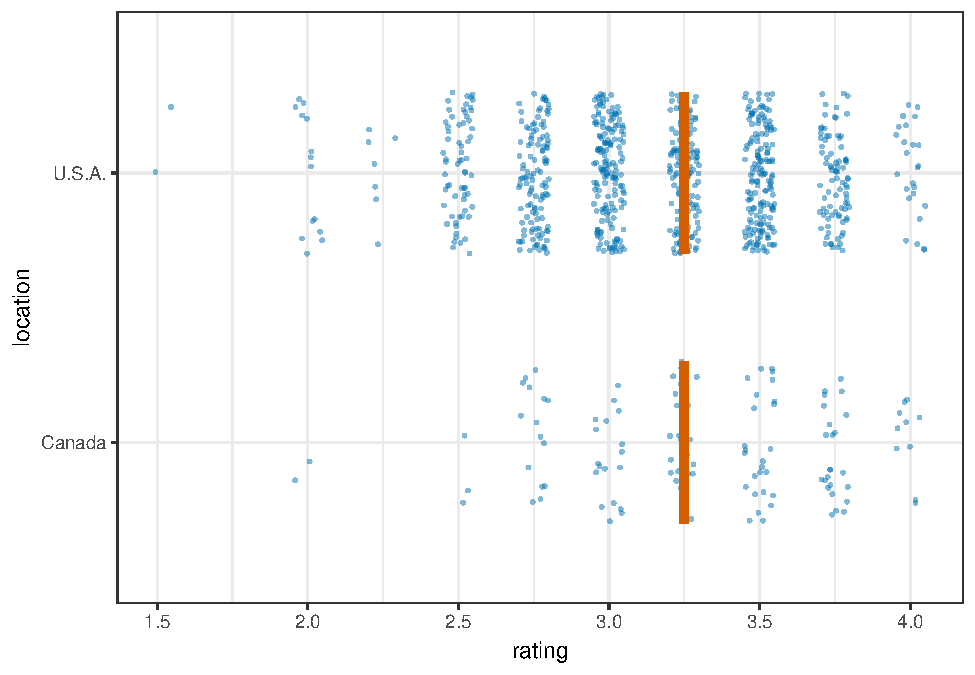
\includegraphics{Intro_Avensik_files/figure-latex/ungeviz-46.pdf} 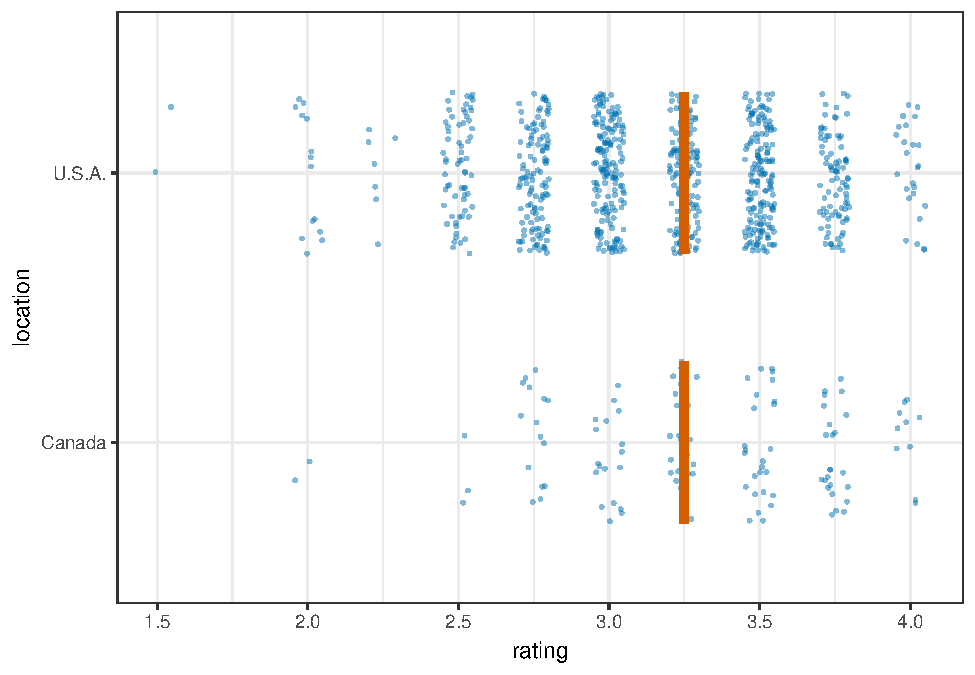
\includegraphics{Intro_Avensik_files/figure-latex/ungeviz-47.pdf} 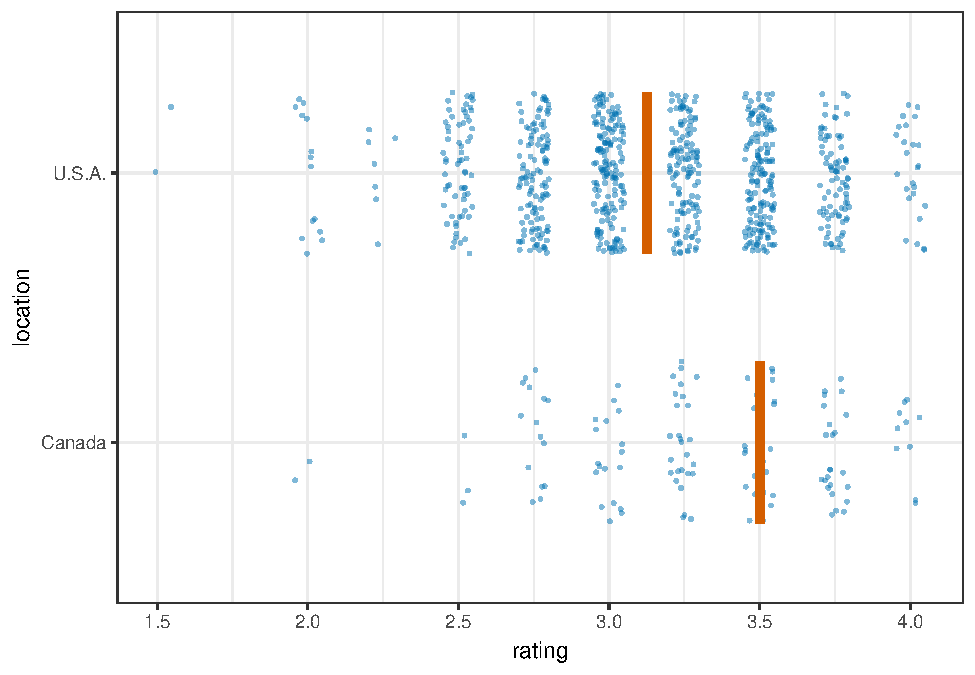
\includegraphics{Intro_Avensik_files/figure-latex/ungeviz-48.pdf} 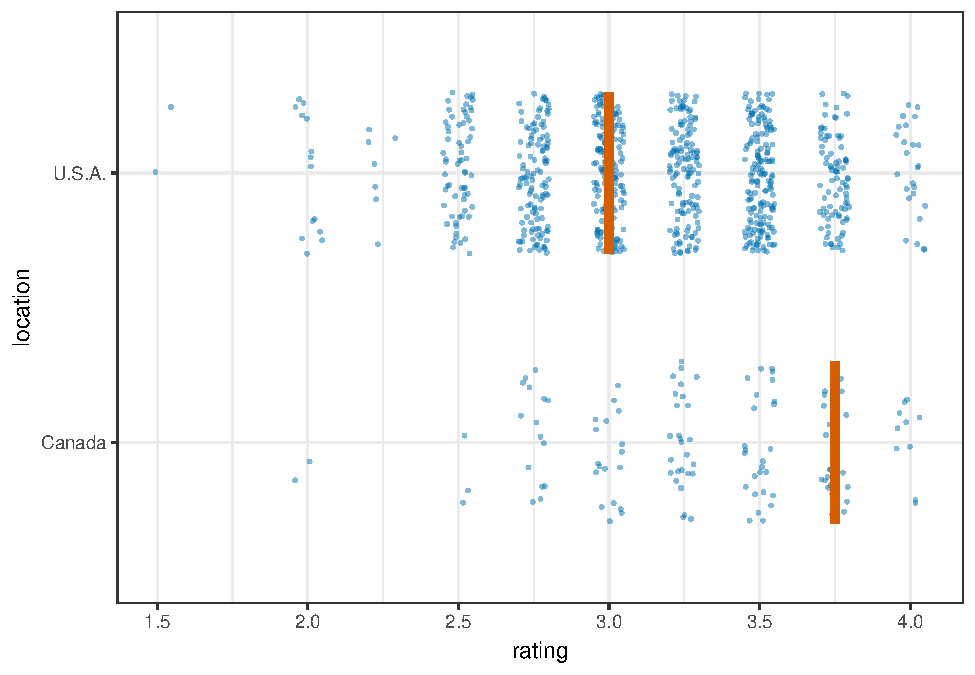
\includegraphics{Intro_Avensik_files/figure-latex/ungeviz-49.pdf} \includegraphics{Intro_Avensik_files/figure-latex/ungeviz-50.pdf} \includegraphics{Intro_Avensik_files/figure-latex/ungeviz-51.pdf} \includegraphics{Intro_Avensik_files/figure-latex/ungeviz-52.pdf} \includegraphics{Intro_Avensik_files/figure-latex/ungeviz-53.pdf} \includegraphics{Intro_Avensik_files/figure-latex/ungeviz-54.pdf} \includegraphics{Intro_Avensik_files/figure-latex/ungeviz-55.pdf} \includegraphics{Intro_Avensik_files/figure-latex/ungeviz-56.pdf} \includegraphics{Intro_Avensik_files/figure-latex/ungeviz-57.pdf} \includegraphics{Intro_Avensik_files/figure-latex/ungeviz-58.pdf} \includegraphics{Intro_Avensik_files/figure-latex/ungeviz-59.pdf} \includegraphics{Intro_Avensik_files/figure-latex/ungeviz-60.pdf} \includegraphics{Intro_Avensik_files/figure-latex/ungeviz-61.pdf} \includegraphics{Intro_Avensik_files/figure-latex/ungeviz-62.pdf} \includegraphics{Intro_Avensik_files/figure-latex/ungeviz-63.pdf} \includegraphics{Intro_Avensik_files/figure-latex/ungeviz-64.pdf} \includegraphics{Intro_Avensik_files/figure-latex/ungeviz-65.pdf} \includegraphics{Intro_Avensik_files/figure-latex/ungeviz-66.pdf} \includegraphics{Intro_Avensik_files/figure-latex/ungeviz-67.pdf} \includegraphics{Intro_Avensik_files/figure-latex/ungeviz-68.pdf} \includegraphics{Intro_Avensik_files/figure-latex/ungeviz-69.pdf} \includegraphics{Intro_Avensik_files/figure-latex/ungeviz-70.pdf} \includegraphics{Intro_Avensik_files/figure-latex/ungeviz-71.pdf} \includegraphics{Intro_Avensik_files/figure-latex/ungeviz-72.pdf} \includegraphics{Intro_Avensik_files/figure-latex/ungeviz-73.pdf} \includegraphics{Intro_Avensik_files/figure-latex/ungeviz-74.pdf} \includegraphics{Intro_Avensik_files/figure-latex/ungeviz-75.pdf} \includegraphics{Intro_Avensik_files/figure-latex/ungeviz-76.pdf} \includegraphics{Intro_Avensik_files/figure-latex/ungeviz-77.pdf} \includegraphics{Intro_Avensik_files/figure-latex/ungeviz-78.pdf} \includegraphics{Intro_Avensik_files/figure-latex/ungeviz-79.pdf} \includegraphics{Intro_Avensik_files/figure-latex/ungeviz-80.pdf} \includegraphics{Intro_Avensik_files/figure-latex/ungeviz-81.pdf} \includegraphics{Intro_Avensik_files/figure-latex/ungeviz-82.pdf} \includegraphics{Intro_Avensik_files/figure-latex/ungeviz-83.pdf} \includegraphics{Intro_Avensik_files/figure-latex/ungeviz-84.pdf} \includegraphics{Intro_Avensik_files/figure-latex/ungeviz-85.pdf} \includegraphics{Intro_Avensik_files/figure-latex/ungeviz-86.pdf} \includegraphics{Intro_Avensik_files/figure-latex/ungeviz-87.pdf} \includegraphics{Intro_Avensik_files/figure-latex/ungeviz-88.pdf} \includegraphics{Intro_Avensik_files/figure-latex/ungeviz-89.pdf} \includegraphics{Intro_Avensik_files/figure-latex/ungeviz-90.pdf} \includegraphics{Intro_Avensik_files/figure-latex/ungeviz-91.pdf} \includegraphics{Intro_Avensik_files/figure-latex/ungeviz-92.pdf} \includegraphics{Intro_Avensik_files/figure-latex/ungeviz-93.pdf} \includegraphics{Intro_Avensik_files/figure-latex/ungeviz-94.pdf} \includegraphics{Intro_Avensik_files/figure-latex/ungeviz-95.pdf} \includegraphics{Intro_Avensik_files/figure-latex/ungeviz-96.pdf} \includegraphics{Intro_Avensik_files/figure-latex/ungeviz-97.pdf} \includegraphics{Intro_Avensik_files/figure-latex/ungeviz-98.pdf} \includegraphics{Intro_Avensik_files/figure-latex/ungeviz-99.pdf} \includegraphics{Intro_Avensik_files/figure-latex/ungeviz-100.pdf}

\hypertarget{analytisk-kemi}{%
\chapter{Analytisk kemi}\label{analytisk-kemi}}

\hypertarget{referenser}{%
\chapter*{Referenser}\label{referenser}}
\addcontentsline{toc}{chapter}{Referenser}

  \bibliography{book.bib,packages.bib}

\end{document}
